\documentclass{article}
\PassOptionsToPackage{numbers,square,comma,sort&compress}{natbib}
\usepackage[main,final]{neurips_2026}
\usepackage[utf8]{inputenc}
\usepackage[T1]{fontenc}
\usepackage{amsmath,amssymb,booktabs,graphicx,microtype,array,url,wrapfig,enumitem}
\makeatletter\newcommand\captionof[1]{\def\@captype{#1}\caption}\makeatother
\usepackage[table]{xcolor}
\usepackage{flafter}
\usepackage{hyperref}
\makeatletter\g@addto@macro\UrlBreaks{\do\-}\makeatother
\hypersetup{colorlinks=true,linkcolor=blue!45!black,citecolor=blue!45!black,urlcolor=blue!45!black}
\setcitestyle{numbers,square,comma,sort&compress}
\newcommand{\tableinput}[1]{\csname @@input\endcsname #1 }
\newcolumntype{P}[1]{>{\raggedright\arraybackslash}p{#1}}
\newcommand{\yes}{$\checkmark$}
\newcommand{\no}{$\times$}
\definecolor{c2shade}{HTML}{E3EEF8}
\definecolor{gateshade}{HTML}{EAF4FB}
\definecolor{verdictshade}{HTML}{EAF7EE}
\definecolor{promptbg}{RGB}{246,246,250}
\newcommand{\codeurl}{\url{https://github.com/koanatakiyo/replicate-independence-llm-agents}}
% Final-size box for a hand-drawn figure that is not drawn yet.
\newcommand{\handdrawn}[3]{\fbox{\parbox[c][#2][c]{\dimexpr#1-2\fboxsep-2\fboxrule\relax}{\centering\footnotesize\textbf{[Hand-drawn figure, to be drawn]}\\[3pt]\itshape #3}}}
\title{Social Interaction Breaks Replicate Independence in Controlled-Clone LLM Agents}
% Author set and order as on the OpenReview submission (Yandan Zheng, Haoran Luo, Anh Tuan Luu).
% Reordering is allowed; additions and removals are not allowed.
% Affiliations and emails still to be supplied by the authors.
\author{%
  Yandan Zheng\\
  Affiliation pending\\
  \texttt{email pending}
  \And
  Haoran Luo\\
  Affiliation pending\\
  \texttt{email pending}
  \And
  Anh Tuan Luu\\
  Affiliation pending\\
  \texttt{email pending}
}

\begin{document}
\maketitle
\begin{abstract}
Multi-agent LLM evaluations and social simulations create many agents from one model and treat them as comparable replicates, even after the agents interact. This assumption has not been tested with matched controls. We test it with SocCogEval, a controlled-clone assay for Social Cognitive Transfer (SCT), and find that it fails. Agents share the same base model, system prompt, and decoding parameters, and a private brief is their only initial difference. A factorial protocol separates the brief, 30 rounds of interaction, and initialization noise, and a matched solo-generation condition bounds the role of extended generation. On Qwen3-122B-FP8, toggling interaction with the briefs held fixed raises off-topic BFI-10 response-profile drift by $\bar{\Delta}{=}{+}0.917$ on Greenfield (95\% CI [+0.620,+1.205], exact $p{=}0.0008$) and ${+}0.912$ on Riverton ([+0.584,+1.255], $p{=}0.0039$), two topically disjoint scenarios. This is about 0.18 Likert points per factor ($g{=}{+}1.07$ and ${+}0.96$). Brief-only controls do not explain the drift. It is directional across runs, persists under temperature-zero re-probing, and stays positive without typed SRM extraction in exploratory tests, so the extractor is not its source. Solo generation accounts for part of the drift, while social interaction remains highest in both scenarios. Across five more model variants, five of ten $(C_2){-}(C_5)$ cells are positive at $\alpha{=}0.05$ with no significant reversal, and all five scenario-averaged $(C_2){-}(C_4)$ contrasts are positive. Interacting clones are not independent replicates unless paired no-interaction controls show otherwise.\footnote{\raggedright Code and data: \codeurl.}
\end{abstract}

\section{Introduction}\label{sec:intro}

\begin{wrapfigure}[15]{r}{0.5\textwidth}
\vspace{-12pt}
\centering
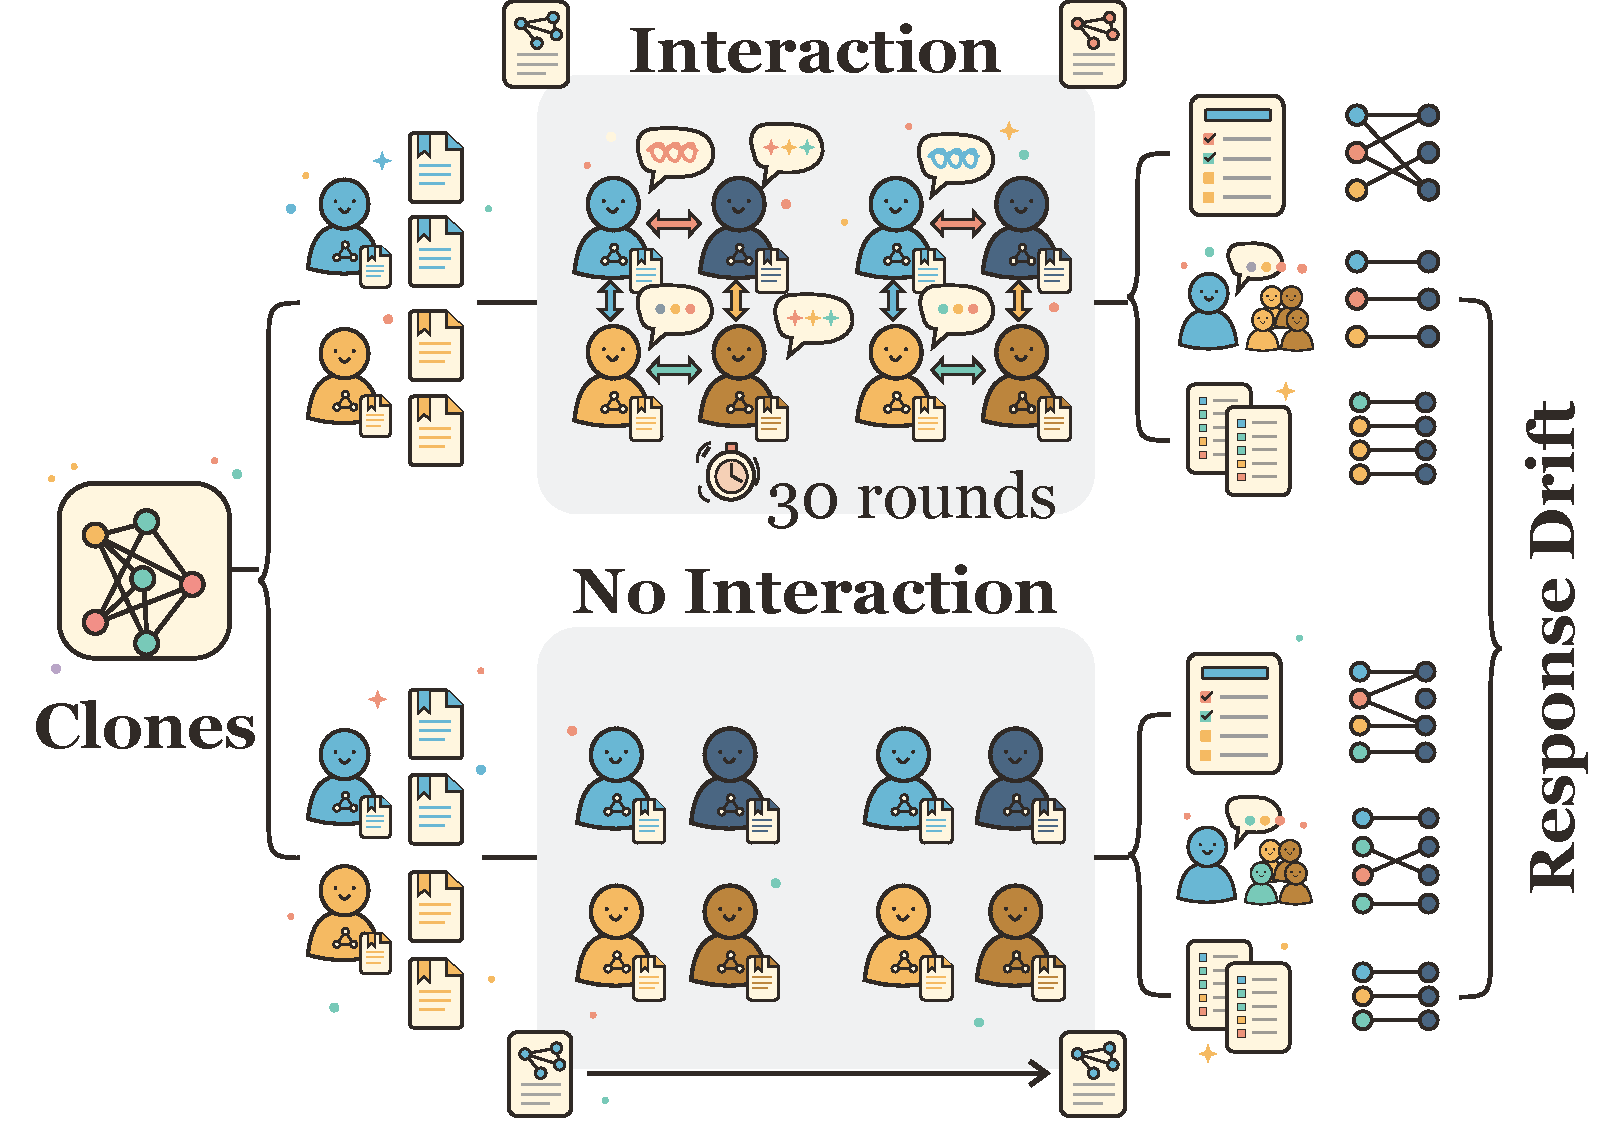
\includegraphics[width=\linewidth]{figures/fig1_teaser.pdf}
\caption{Interaction moves off-topic profiles.}\label{F0}
\vspace{-10pt}
\end{wrapfigure}

Many LLM systems build a population from copies of one model, including multi-agent debate~\citep{Du2024_MultiagentDebate,Liang2024_DivergentDebate,Du2024_Debate,Smit2024_MAD}, collaboration and evaluation frameworks~\citep{Li2023_CAMEL,Wu2024_AutoGen,Hong2024_MetaGPT,Chan2024_ChatEval}, simulated survey samples~\citep{Argyle2023,Aher2023_SimulateHumans}, and simulations of conflict, opinion, cooperation, and whole societies~\citep{Hua2024_WarAgent,OASIS,AgentSociety,Generative_Agents,Park2024_1000,Concordia,Li2024_SocioVerse,Chuang2024_OpinionDynamics,CisnerosVelarde2025_Funding,Piatti2024_GovSim,FlintAshery2025_Conventions,Anthis2025_SocialSim}. These studies treat the copies as comparable replicates of one system, even after many rounds of talk. If interaction changes the agents, each interacting population is one sample, and counting agents or posts as independent observations overstates the evidence~\citep{Hurlbert1984,Miller2024_ErrorBars}.

\begin{figure}[t]
\centering
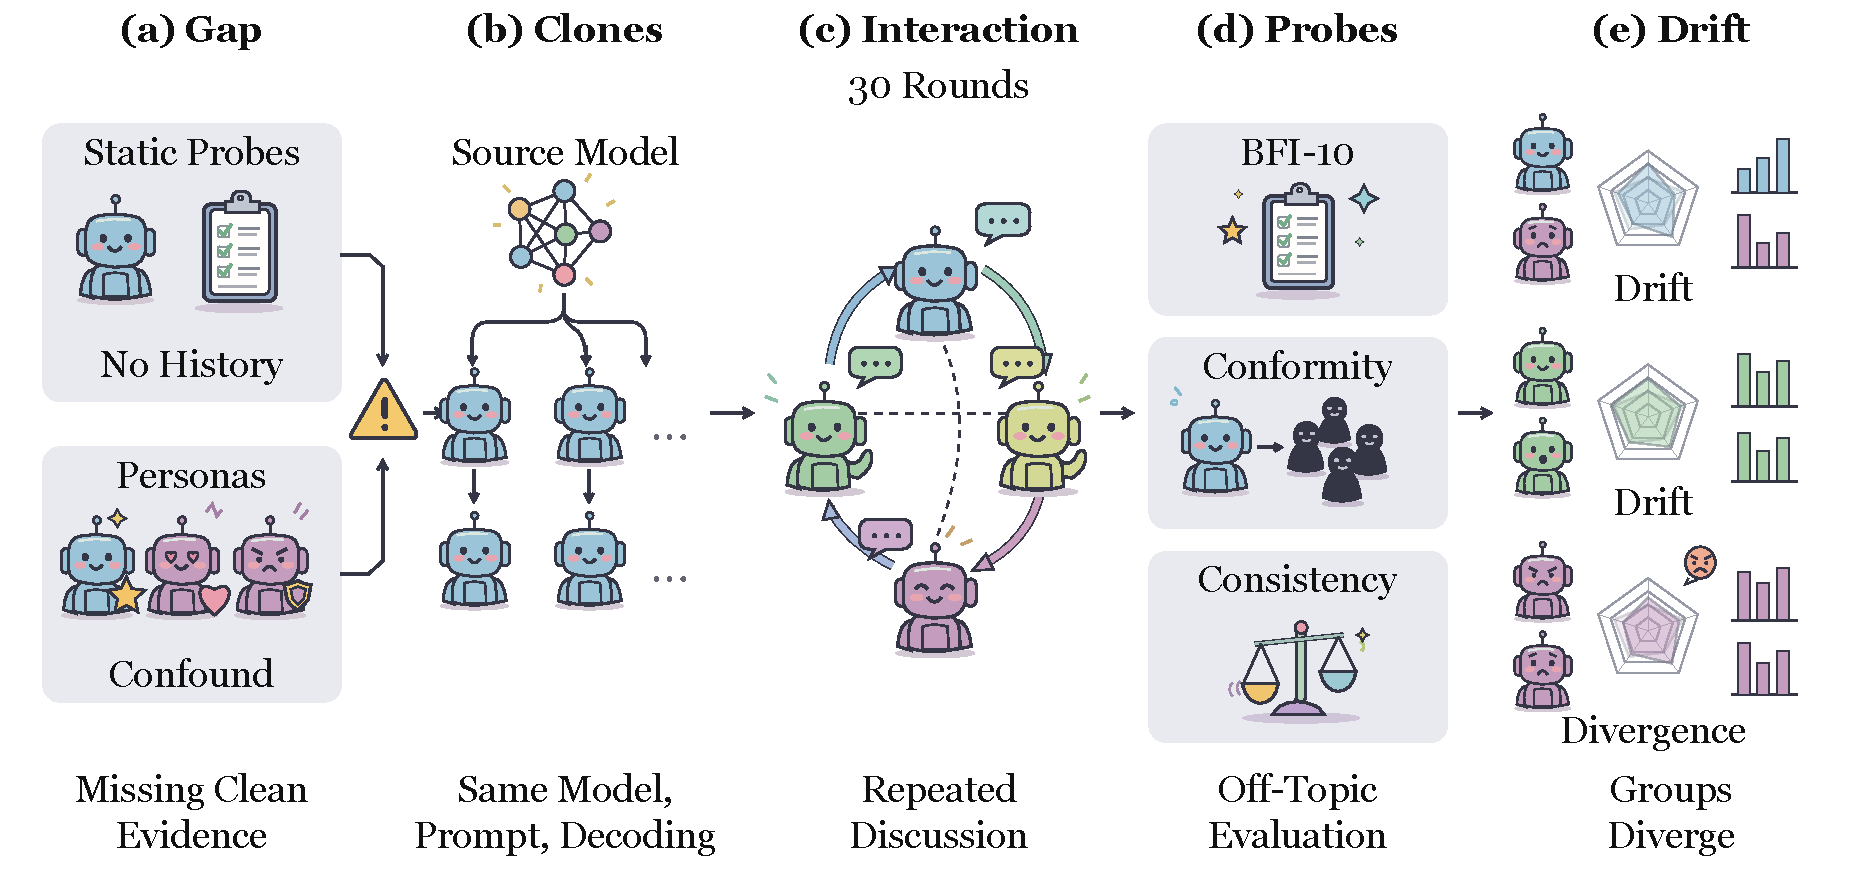
\includegraphics[width=\textwidth]{figures/fig2_overview.pdf}
\caption{The evaluation gap (a) and how SocCogEval tests transfer to unrelated probes (b--e).}\label{F1}
\end{figure}


This assumption still lacks a controlled test (Figure~\ref{F1}). Benchmarks score a frozen model on curated items or a short episode~\citep{MT-bench,AgentBench,ToMBench,Kim2023_FANTOM,Xu2024_OpenToM,CogBench,CogMir,PsychoBench}. Social simulations run long interactions but assign personas or opinions at the start, which mixes injected priors with the effect of interaction. Studies of drift, stability, and conformity measure the discussed task or the dialog itself~\citep{Li2024_PersonaDrift,Laban2025_LostMultiTurn,Kovac2024_StickToRole,Weng2025_Conformity,Potter2026,Rath2026_AgentDrift}, and personalities can emerge when undifferentiated agents communicate~\citep{Takata2024}. A controlled test has to meet three challenges. It must inject no differences at initialization, separate the effect of a brief from the effect of interaction, and use a probe unrelated to the discussed topic, analyzed at the level of the run.

SocCogEval meets them with controlled clones that share base model, system prompt, and decoding parameters, each holding at most one private brief. The Factorial Social Interaction Protocol (FSIP) crosses brief presence with 30 rounds of interaction, so the pure-interaction contrast $(C_2){-}(C_4)$ holds the brief fixed and toggles interaction (Figure~\ref{F0}). A solo-generation condition $C_6$ matches the call budget without any partner. The measurements follow three nested questions: do clones diverge on the discussed decision, do they predict exposed in-group peers better, and does the divergence transfer to an off-topic BFI-10 response profile?

\begin{figure}[t]
\centering
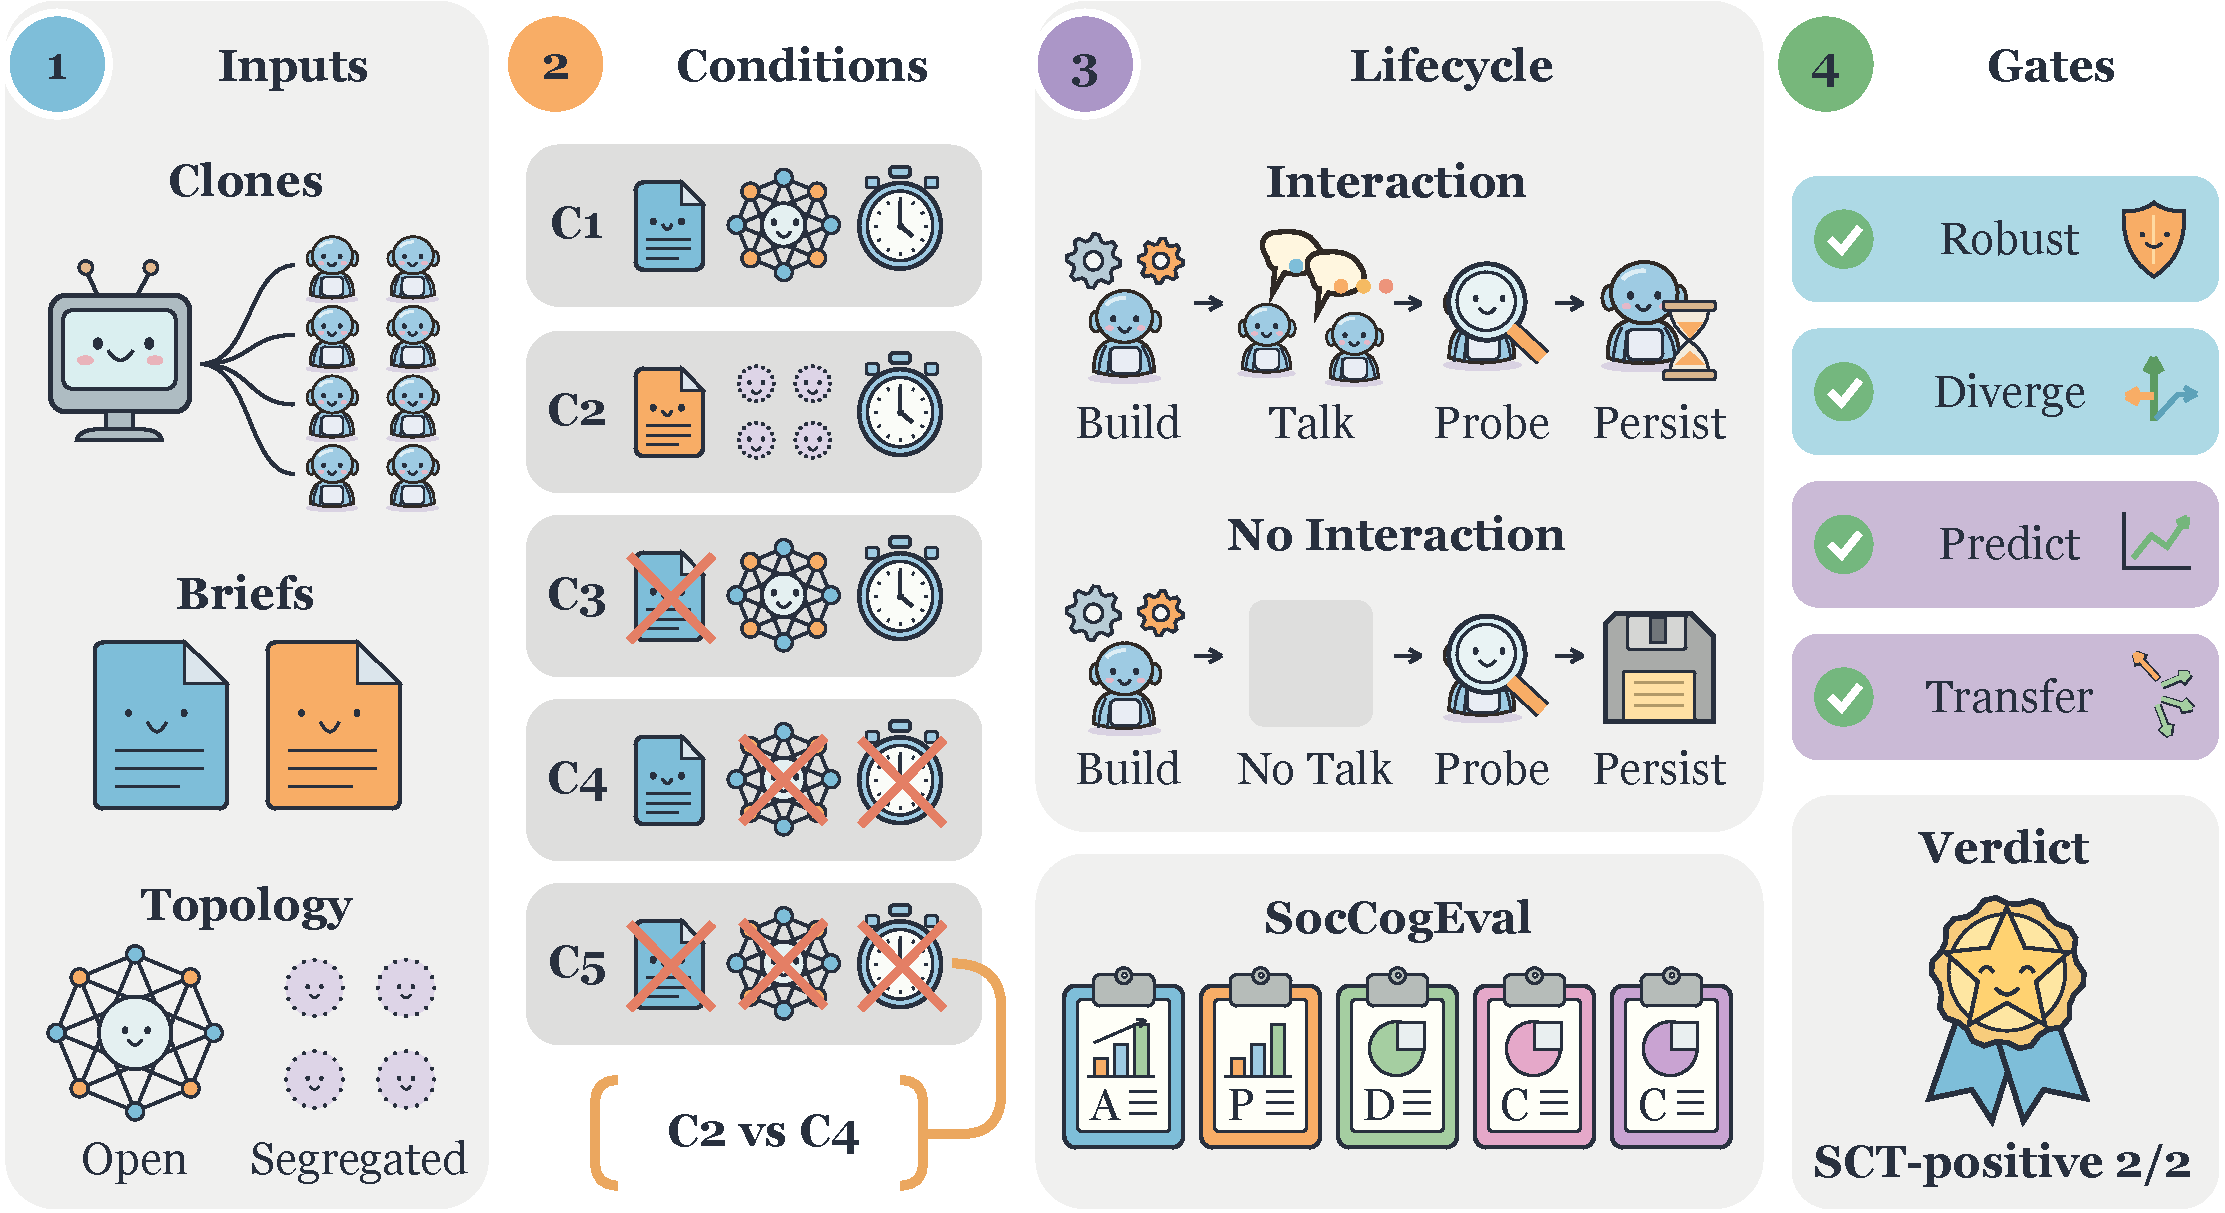
\includegraphics[width=\textwidth]{figures/fig3_fsip.pdf}
\caption{FSIP design and SocCogEval pipeline: $(C_2){-}(C_4)$ fixes the brief and toggles interaction.}\label{F2}
\end{figure}


Social interaction breaks replicate independence on the primary transfer outcome. On Qwen3-122B-FP8, the pure-interaction contrast is $\bar{\Delta}{=}{+}0.917$ BFI-10 L1 units on Greenfield and ${+}0.912$ on Riverton (run-level $p{=}0.0008$ and $0.0039$, $g{\approx}1.0$), about 0.18 Likert points per factor. Brief alone does not explain it, and it survives deterministic re-probing and a verbatim-history ablation without typed memory extraction. Solo generation reproduces part of the shift, while social interaction remains highest in both scenarios. Five more model variants give positive but uneven breadth, and all five have positive scenario-averaged $(C_2){-}(C_4)$ contrasts.

Our contributions are fourfold. (i) We define the Social Cognitive Transfer (SCT) task with three nested sub-tasks, Decision, Prediction, and Transfer. (ii) We propose FSIP, a five-condition design that isolates initialization noise, brief alone, interaction given brief, and brief given interaction, with a matched solo-generation condition $C_6$ as the mechanism boundary. (iii) We introduce SocCogEval, which combines task probes, a primary BFI-10 transfer instrument~\citep{Rammstedt2007_BFI10,PsychoBench}, secondary conformity and consistency probes~\citep{Asch1956_Conformity,CogMir}, and a contrast schema that turns measurements into causal claims. (iv) We show that social interaction breaks replicate independence on the primary transfer outcome, with cross-scenario stability and positive cross-model direction. The reported drift is restricted to Part 2 instruments unrelated to the discussion and gated by a three-part criterion (Section~\ref{sec:metrics}). SocCogEval is an identification protocol for this drift, not a benchmark of social-cognition capacity, and the drift is post-interaction response-profile drift, not personality change (Section~\ref{sec:exp-limits}).

\section{Related Work}\label{sec:related}

\textbf{Social-cognition and psychometric evaluation.} ToMBench~\citep{ToMBench}, FANToM~\citep{Kim2023_FANTOM}, OpenToM~\citep{Xu2024_OpenToM}, CogMir~\citep{CogMir}, CogBench~\citep{CogBench}, and PsychoBench~\citep{PsychoBench} score frozen models on curated items. Psychometric frameworks measure and shape LLM personality~\citep{SerapioGarcia2025_PsychometricLLM,Ye2025_LLM_Psychometrics}, expressed values shift with context~\citep{Kovac2024_StickToRole}, and the reliability of self-report inventories for LLMs is contested~\citep{Binz2023,Shu2024_PsychReliability,Gupta2024_SelfAssessment,Huang2024_ScaleReliability,Lee2025_TRAIT,Jiang2024_PersonaLLM,Han2025_PersonalityIllusion}. These works measure a snapshot and cannot separate what is in the weights from what an interaction history adds. SocCogEval places BFI-10~\citep{Rammstedt2007_BFI10,PsychoBench} and Asch-style items~\citep{Asch1956_Conformity} in a paired pre-post design, so scores become difference-in-differences statistics that read as transfer.

\textbf{Agent societies and multi-agent systems.} OASIS~\citep{OASIS}, AgentSociety~\citep{AgentSociety}, generative-agent worlds~\citep{Generative_Agents,Park2024_1000}, Concordia~\citep{Concordia}, SocioVerse~\citep{Li2024_SocioVerse}, and WarAgent~\citep{Hua2024_WarAgent} simulate LLM populations in which opinions~\citep{Chuang2024_OpinionDynamics,CisnerosVelarde2025_Funding}, cooperation~\citep{Piatti2024_GovSim}, conventions~\citep{FlintAshery2025_Conventions}, and individual personalities~\citep{Takata2024} emerge. SOTOPIA scores social skill within an episode~\citep{Zhou2024_SOTOPIA}, and LLM simulation is proposed as a social-science method~\citep{Anthis2025_SocialSim,Mou2024_SocialSimSurvey}. Debate, evaluation, and collaboration frameworks build teams from one model~\citep{Du2024_MultiagentDebate,Liang2024_DivergentDebate,Du2024_Debate,Smit2024_MAD,Chan2024_ChatEval,Li2023_CAMEL,Wu2024_AutoGen,Hong2024_MetaGPT}, often with persistent memory~\citep{MemGPT,Xu2025_AMEM,Mem0}. These studies inject heterogeneous priors or report collective outcomes, so they cannot isolate what interaction does to each agent. Controlled clones and a factorial contrast schema remove that confound.

\textbf{Drift, stability, and conformity.} Instructions fade within a dialog~\citep{Li2024_PersonaDrift}, reliability drops over multi-turn conversations~\citep{Laban2025_LostMultiTurn}, models agree with interlocutors~\citep{Sharma2024_Sycophancy} and conform to majorities~\citep{Weng2025_Conformity}, multi-agent systems fail through coordination errors~\citep{Cemri2025_MASFailures}, and a peer's presence changes behavior~\citep{Potter2026}. Rath~\citep{Rath2026_AgentDrift} defines drift as progressive degradation of task quality, coordination, and inter-agent coherence through a twelve-component Agent Stability Index. These works measure instability on the task or in the dialog (human parallels in Appendix~\ref{app:related}). We instead test distributional exchangeability of bit-identical clones. Initialization and brief assignment stay fixed, and we ask whether interaction transfers to off-topic response profiles under matched brief-only and no-interaction controls.

\textbf{Uncertainty in evaluation.} Observations within one unit are not independent replicates~\citep{Hurlbert1984}, items that share a source need clustered errors~\citep{Miller2024_ErrorBars,Cameron2015}, and synthetic samples can understate variation~\citep{Bisbee2024}. Multi-turn agent evaluation has mostly targeted task success~\citep{Yao2023_ReAct,MT-bench,AgentBench}. We treat the run as the unit of replication.

\begin{figure}[t]
\centering
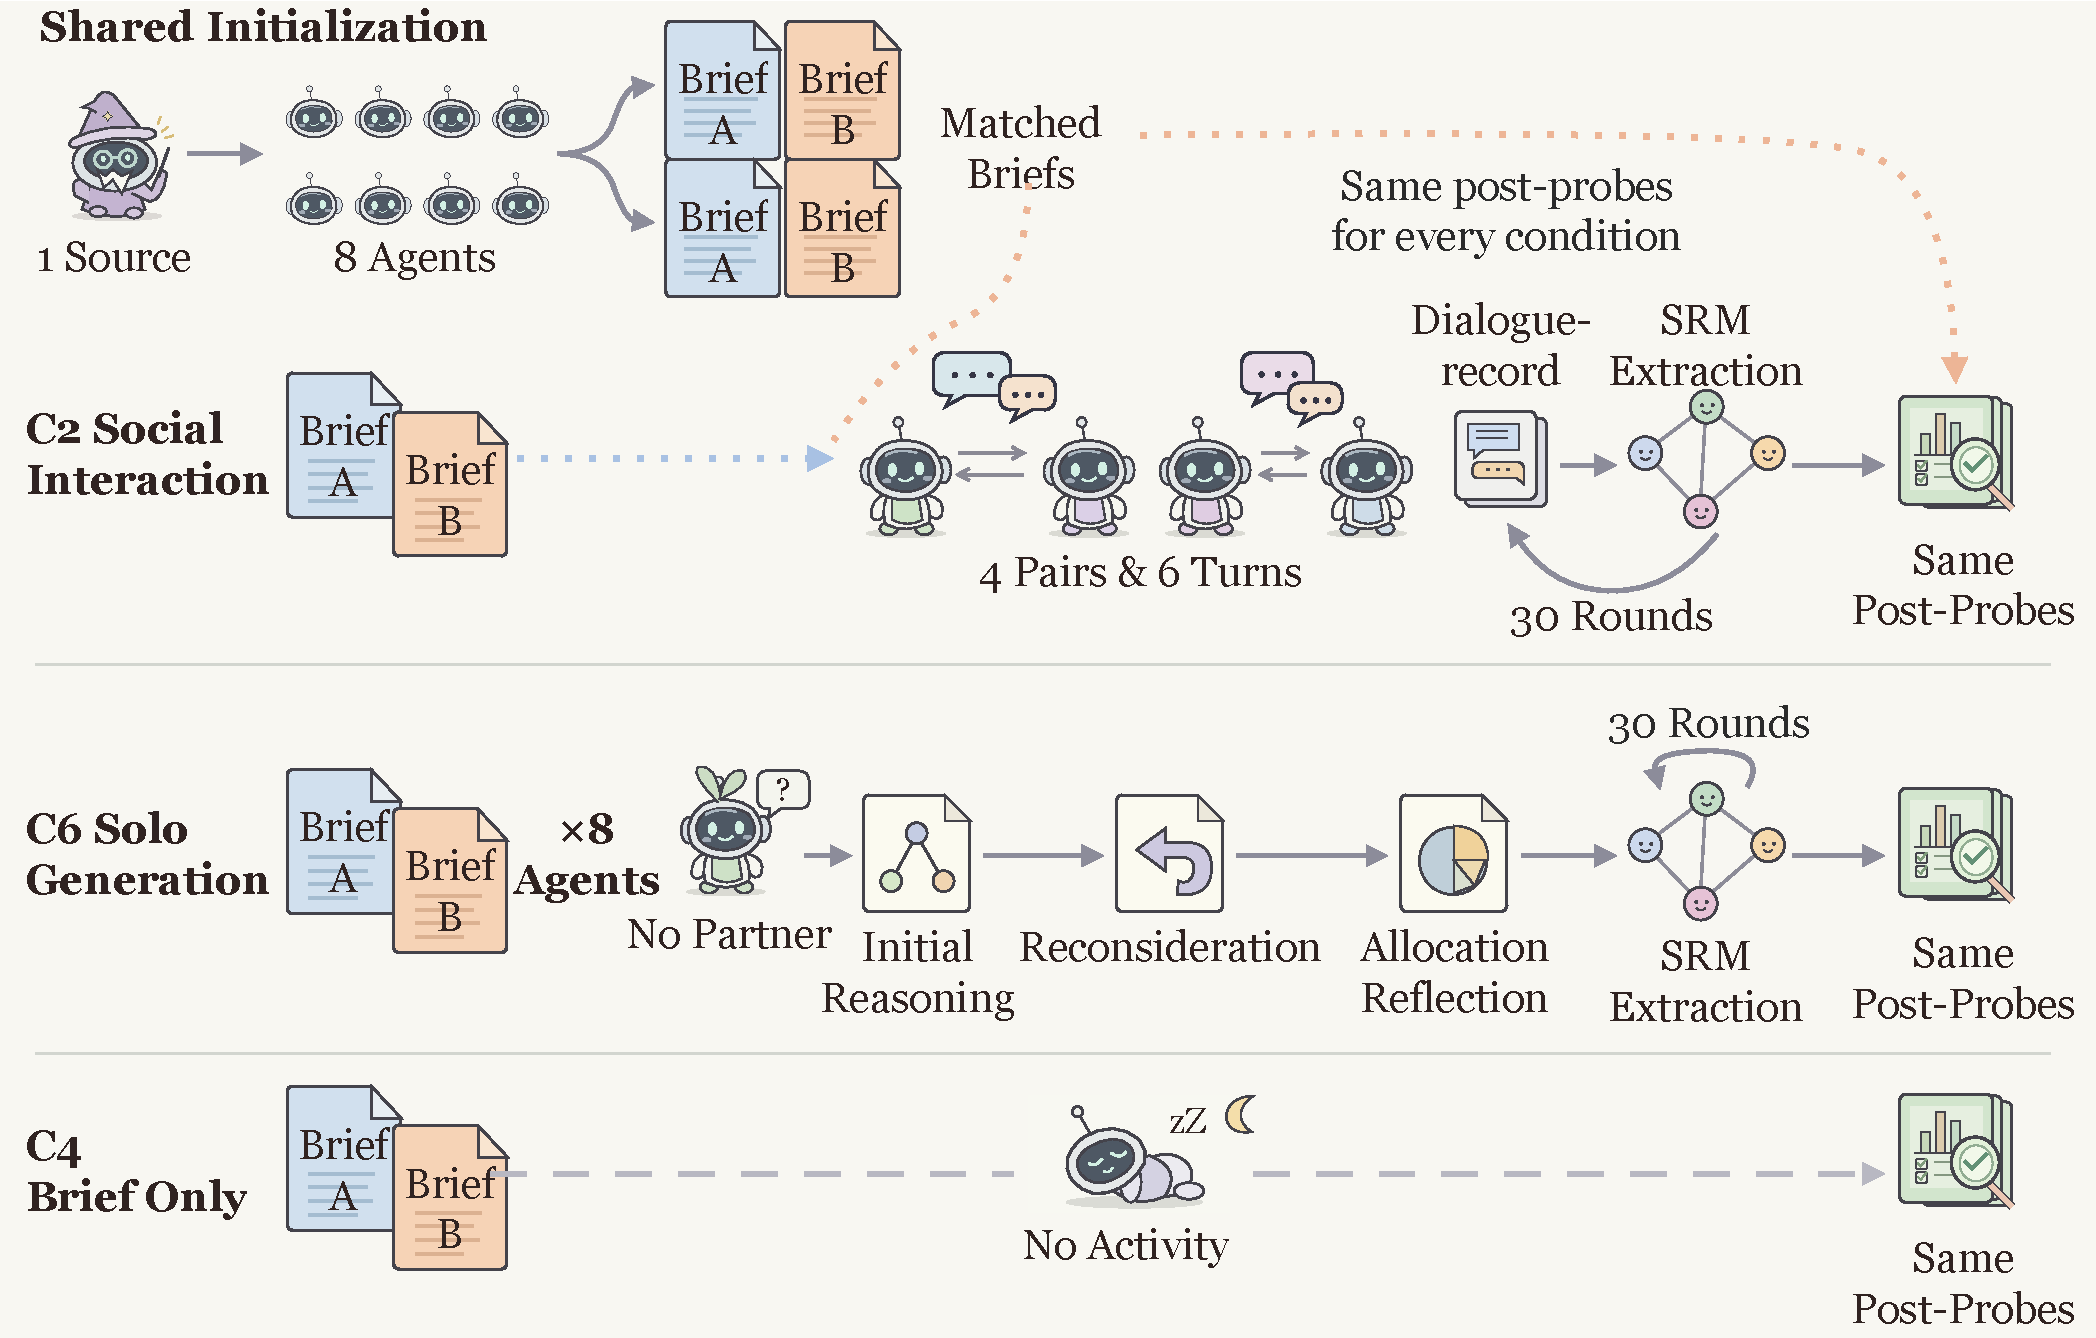
\includegraphics[width=\textwidth]{figures/fig4_c6.pdf}
\caption{The three comparison lanes. $C_6$ matches the $C_2$ call budget without a partner.}\label{F3sch}
\end{figure}

\section{SocCogEval: Task, Protocol, and Measurement}\label{sec:method}\label{sec:task}

SocCogEval combines a task definition, a factorial protocol, and a measurement suite. The task defines what would count as social cognitive transfer. The protocol separates interaction from briefs, initialization noise, and memory machinery. The measurements convert each run into contrast-level evidence.

\subsection{Task: Decision, Prediction, Transfer}\label{sec:sct-task}

An SCT instance specifies a frozen base model $M$, an agent population $A{=}\{a_1, \dots, a_k\}$ of $k$ clone agents that share system prompt and decoding parameters, an interaction graph $G$ over $A$ (all-to-all, two-component segregated, or empty), a scenario $S$ with a 5-dim allocation space, an optional brief assignment $T$ (asymmetric A and B, symmetric A, or none), and an interaction horizon $N$ (default 30 rounds). The clone constraint is the load-bearing one. In any condition without briefs, $a_i$ and $a_j$ have bit-identical initial state. When briefs are assigned, the only initial difference is the private brief document. Three nested questions follow. SCT-Decision asks whether post-interaction allocation in segregated, asymmetrically briefed conditions diverges beyond what brief alone or initialization noise produce. SCT-Prediction asks whether agents in segregated conditions predict in-group members more accurately than out-group members. SCT-Transfer asks whether the divergence appears on instruments topically unrelated to the discussion, after subtracting the no-interaction baseline.

\subsection{Factorial Social Interaction Protocol}\label{sec:fsip}

The factorial axes are brief ($T \in \{\text{none}, \text{A only}, \text{asymmetric A and B}\}$) and interaction ($N \in \{0, 30\}$ with topology $G \in \{\text{open}, \text{segregated}\}$). The design uses five conditions plus one mechanism control (Figure~\ref{F2}). $C_1$ (open, symmetric brief) uses an all-to-all topology in which every agent receives Brief A, as an open-network reference. $C_2$ (segregated, asymmetric brief) splits agents into two components, half with Brief A and half with Brief B, and is the headline condition. $C_3$ (segregated, no brief) keeps the $C_2$ topology without briefs and isolates interaction alone. $C_4$ (brief only) assigns the A and B briefs with $N{=}0$ and isolates brief alone. $C_5$ (no brief, no interaction) sets the initialization noise floor. $C_6$ (solo generation) keeps the $C_2$ briefs, memory policy, probe cadence, and logical call budget, with private generation in place of partners (Figure~\ref{F3sch}).

The load-bearing causal contrast is $(C_2){-}(C_4)$ on every measured outcome. It holds the brief fixed, since both conditions use asymmetric A and B briefs, and toggles 30 rounds of interaction on or off. Interaction-created history, memory, and elapsed conversation are post-treatment pathways through which the treatment acts, so $(C_2){-}(C_4)$ is the total effect of interaction given the same brief in this protocol. One scope limit matters. $C_1$ uses symmetric briefs while $C_2$ uses asymmetric briefs, so the $(C_2){-}(C_1)$ contrast varies brief-symmetry and topology jointly and does not isolate topology. We therefore exclude topology from the causal claims and report $(C_2){-}(C_1)$ only as a descriptive comparison. Replica counts per condition are $\{C_1{=}7, C_2{=}8, C_3{=}5, C_4{=}5, C_5{=}3, C_6{=}5\}$ per scenario, with $k{=}8$ agents per replica.

\textbf{Solo-generation control.} $C_6$ gives each agent three private generation calls per round (initial reasoning, reconsideration, allocation reflection) and one memory extraction, with no partner identity, messages, or feedback. This yields 720 content and 240 extraction calls per run, matching $C_2$'s intended logical totals. Its design was frozen before formal outcomes were examined, and all ten formal $C_6$ runs passed audit (Appendix~\ref{app:c6}). $(C_6){-}(C_4)$ measures the solo-generation shift, and $(C_2){-}(C_6)$ compares social and solo histories.

\subsection{Scenarios, Runtime Cycle, and Models}\label{sec:fsip-cycle}

We run two topically disjoint scenarios. Greenfield is a community-grant allocation problem with \$10M across five categories such as Education, Healthcare, and Infrastructure. Riverton is a workforce transition budget problem with \$5M across categories such as Automation and Workforce Training. Both use 5-dim allocation vectors so Part 1 metrics are commensurable. Both have softened A and B briefs that frame the same problem through moderately divergent value lenses (Appendix~\ref{app:scenarios}). Per-round mechanics follow a Build-Talk-Probe-Persist cycle. Build updates a typed Social-Relational Memory (SRM) hypergraph from the previous round's conversations. Talk forms 4 random pair conversations among 8 agents with 6 turns each. Probe runs SocCogEval instruments at predetermined cadences, with belief and common-ground probes every five rounds that leave conversation history and memory unchanged. Persist writes the round artifacts to disk.

\textbf{Models and filtering.} The primary model is Qwen3-122B-FP8~\citep{Qwen2025_Qwen3} served locally via vLLM. Five model variants run on $\{C_2, C_4, C_5\}$ in both scenarios, three runs per condition and scenario: Qwen3-VL-32B-Instruct~\citep{Qwen2025_Qwen3VL} run text-only, DeepSeek-V3~\citep{DeepSeekAI2024_DeepSeekV3}\footnote{Historical DeepSeek $C_2$ runs used the provider identifier \texttt{deepseek-chat} and the added $C_4$ runs used \texttt{deepseek-v4-flash}. Exact provider revisions were not recorded (Appendix~\ref{app:routing}).}, GPT-4.1-mini~\citep{OpenAI2025_GPT41}, Gemini-2.5-Flash~\citep{GoogleDeepMind2025_Gemini25}, and Llama-4-Scout~\citep{MetaAI2025_Llama4}. Figures abbreviate the six models as Q-122B, Q-VL, DS-V3, GPT-mini, Gem-Flash, and L4-Scout. The selected dataset contains 168 runs: 56 primary, 90 cross-variant, 12 no-SRM, and 10 $C_6$. Primary factorial analyses use a strict run-id filter so cross-variant replicas cannot enter the within-Qwen3-122B-FP8 baseline. Content generation uses temperature 0.7, BFI-10 and conformity use 0.7, and allocation, prediction, and memory extraction use 0.

\subsection{Measurements and Statistics}\label{sec:metrics}

Among the Part 2 instruments, we designate BFI-10 response-profile drift as the primary transfer outcome. It is topic-independent, compact, and inherited from classical BFI-10 psychometrics and prior LLM psychometric evaluation work~\citep{Rammstedt2007_BFI10,PsychoBench,SerapioGarcia2025_PsychometricLLM,Ye2025_LLM_Psychometrics}. BFI-10 is manuscript-designated primary, without an external timestamped preregistration. The claim does not require the inventory to be psychometrically valid for LLMs in the human sense. We use its fixed item structure as an off-topic response-profile probe whose items are unrelated to either allocation scenario. Conformity and cross-prompt consistency are secondary transfer instruments, using Asch-style conformity materials and CogMir-inspired probe phrasing~\citep{Asch1956_Conformity,CogMir}. Allocation divergence and prediction MAE are the Part 1 instruments and support the Decision and Prediction parts of the SCT route (scoring formulas in Appendix~\ref{app:stats}).

For agent $i$ in run $r$, let $s_{rif}^{t}$ be the score of BFI factor $f$ at phase $t\in\{\mathrm{pre},\mathrm{post}\}$, after reverse-scoring items 1, 3, 4, 5, and 7. Agent drift, run-mean drift, the contrast between conditions, and the signed factor contrast are
\begin{equation}\label{eq:drift}
 d_{ri}=\sum_{f=1}^{5}\bigl|s_{rif}^{\mathrm{post}}-s_{rif}^{\mathrm{pre}}\bigr|,\quad
 D_r=\tfrac{1}{8}\sum_{i}d_{ri},\quad
 \bar\Delta_{a,b}=\overline D_{C_a}-\overline D_{C_b},\quad
 \kappa_f=\overline m_{C_2,f}-\overline m_{C_4,f},
\end{equation}
where $m_{rf}=\frac{1}{8}\sum_i(s_{rif}^{\mathrm{post}}-s_{rif}^{\mathrm{pre}})$. Because $d_{ri}$ sums five factor-level shifts, $\bar\Delta{=}0.92$ corresponds to about 0.18 Likert points per factor. Unsigned L1 can grow through directional movement or dispersion, so $\kappa_f$ and run-level variance ratios report direction and spread separately.

\textbf{Unit of analysis.} Agents in one run share an evolving history and interfere with each other's outcomes~\citep{Hudgens2008,Aronow2017}, so the run is the independent unit for the primary inference and agents within a run are not replicates~\citep{Hurlbert1984}. Each run is summarized by $D_r$. Conditions are compared with two-sided exact permutation tests that enumerate all label allocations, so no Monte Carlo correction is needed~\citep{Phipson2010}, and with run-bootstrap 95\% intervals~\citep{Efron1979}. Raw $\bar\Delta$ leads the reporting. Hedges' $g$ with the small-sample correction~\citep{Hedges1981} is secondary, and we report it as undefined when the pooled within-condition SD falls below 0.05 in the metric's native units. The gate status in Table~\ref{tab:gates} keeps the original agent-stratified two-level cluster bootstrap, which resamples replicas and then agents within each replica (10{,}000 resamples), with Welch's $t$ as the parametric reference.

\textbf{Reporting standard.} The primary SCT-positive claim is made for BFI-10 response-profile drift. It requires three criteria. First, a Part 1 allocation contrast must clear the majority-of-dimensions rule on $(C_2){-}(C_5)$. Second, BFI-10 must clear its CI gate on $(C_2){-}(C_5)$. Third, BFI-10 must clear its CI gate on the pure-interaction $(C_2){-}(C_4)$. Secondary instruments get the same gate status but serve as scenario-specific supporting evidence, not the load-bearing claim.

\section{Experiments}\label{sec:exp}\label{sec:exp-setup}

We organize the results around seven questions. \textbf{RQ1}: does interaction given the same brief shift off-topic responses? \textbf{RQ2}: does the shift survive changes to memory, probe temperature, and partner presence? \textbf{RQ3--RQ5}: does the SCT route hold from Decision through Prediction to Transfer? \textbf{RQ6}: does the direction extend across model variants, and what does it imply for replication? \textbf{RQ7}: what does the clearest scenario look like along the whole route?

\subsection{RQ1: Does Interaction Given the Same Brief Shift Off-Topic Responses?}\label{sec:exp-main}

\begin{table}[t]
\centering\footnotesize
\setlength{\tabcolsep}{3.2pt}
\caption{FSIP decomposition. Only pure interaction is large and significant in both scenarios.}\label{tab:decomp}
\resizebox{\textwidth}{!}{%
\begin{tabular}{llc rrrr rrrr}
\toprule
& & & \multicolumn{4}{c}{Greenfield} & \multicolumn{4}{c}{Riverton} \\
\cmidrule(lr){4-7}\cmidrule(lr){8-11}
Contrast & Isolates & Gate & $\bar\Delta$ & $g$ & 95\% CI & $p$ & $\bar\Delta$ & $g$ & 95\% CI & $p$ \\
\midrule
\tableinput{tables/t1_decomp.tex}
\bottomrule
\end{tabular}}
\end{table}

\begin{figure}[t]
\centering
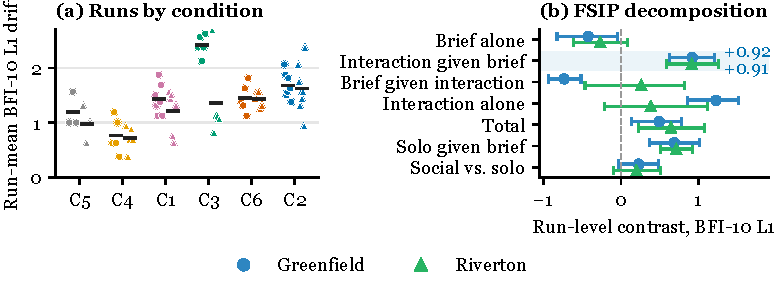
\includegraphics[width=\textwidth]{figures/fig4_primary.pdf}
\caption{Run-level drift (a) and FSIP decomposition (b). $C_2$ exceeds $C_4$ in both scenarios.}\label{fig:primary}
\end{figure}

\textbf{Finding 1: the pure-interaction contrast clears all three gates in both scenarios.} As Table~\ref{tab:decomp} shows, controlled clones with the same private-brief assignment but no interaction differ from clones with the same assignment and 30 rounds of interaction by $\bar{\Delta}{=}{+}0.917$ (Greenfield) and ${+}0.912$ (Riverton) BFI-10 L1 units, with exact run-level $p{=}0.0008$ and $0.0039$ and $g{\approx}1.0$ on both. Because BFI-10 L1 sums five factor-level absolute shifts, this corresponds to about 0.18 Likert points per factor. All eight Greenfield $C_2$ run means exceed the largest $C_4$ mean, and in Riverton seven exceed it and one ties it (Figure~\ref{fig:primary}a). The headline result does not depend on the thinner $C_5$ baseline. The two scenarios are topically disjoint (a community grant and a workforce transition). The BFI-10 items~\citep{Rammstedt2007_BFI10,PsychoBench} are unrelated to either scenario, and the magnitude is near-identical across them. This is the cross-task, cross-scenario stability signature that would be hard to obtain from any mechanism reducible to surface opinion change on the discussed topic.

\textbf{Finding 2: brief alone does not explain the drift.} A brief, a noisy no-interaction baseline, or a probe artifact could in principle produce the BFI-10 shift without interaction. Figure~\ref{fig:primary}b rules out the brief. The brief-alone contrast $(C_4){-}(C_5)$ is small and negative on Greenfield ($\bar{\Delta}{=}{-}0.43$) and trends negative on Riverton without significance. In contrast, $(C_2){-}(C_4)$ stands roughly $1.2{-}1.3$ BFI L1 units above the brief-alone row. Interaction without any brief asymmetry is also sufficient on at least one scenario, since $(C_3){-}(C_5)$ is significantly positive on Greenfield and trends positive on Riverton. Among the five FSIP contrasts, only $(C_2){-}(C_4)$ is positive, large, and significant in both scenarios.

The BFI-10 result remains a response-profile drift on a human-derived inventory, not evidence of human-like personality change. Still, three observations make trivial accounts too small. First, the headline contrast holds asymmetric briefs fixed. Second, the no-SRM ablation (RQ2) keeps the drift positive without the typed SRM extractor. Third, the same interaction protocol produces structured Decision and Prediction effects (RQ3--RQ5), which is not what one would expect from random sampling drift alone.

\subsection{RQ2: Does the Shift Survive Memory, Temperature, and Partner Changes?}\label{sec:exp-srm}

\begin{figure}[t]
\begin{minipage}[c]{0.56\textwidth}
\centering\footnotesize
\setlength{\tabcolsep}{2.4pt}
\captionof{table}{Setting ablations. Every contrast stays positive (raw $\bar\Delta$, exact $p$).}\label{tab:settings}
\begin{tabular}{llrrrr}
\toprule
& & \multicolumn{2}{c}{Greenfield} & \multicolumn{2}{c}{Riverton} \\
\cmidrule(lr){3-4}\cmidrule(lr){5-6}
Setting & Contrast & $\bar\Delta$ & $p$ & $\bar\Delta$ & $p$ \\
\midrule
\tableinput{tables/t2_settings.tex}
\bottomrule
\end{tabular}
\end{minipage}\hfill
\begin{minipage}[c]{0.41\textwidth}
\centering
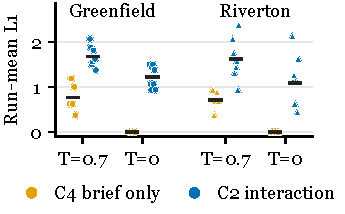
\includegraphics[width=\linewidth]{figures/fig5_t0.pdf}
\captionof{figure}{$C_2$ stays above $C_4$ at BFI $T{=}0.7$ and $T{=}0$.}\label{fig:t0}
\end{minipage}
\end{figure}

\textbf{Finding 3: the shift survives deterministic re-probing.} We re-probed every frozen primary $C_2$ and $C_4$ state at BFI temperature zero, without generating new interaction trajectories. The raw contrast remains $+1.227$ on Greenfield and $+1.094$ on Riverton (Table~\ref{tab:settings}), with all 8/8 $C_2$ run means positive in both scenarios (Figure~\ref{fig:t0}). At $T{=}0$, $C_4$ produces the same pre/post score under its identical prompt, giving a deterministic zero, so raw differences are the informative scale. The same leading signed factors keep 8/8 directional agreement: Greenfield extraversion $+0.344$ and neuroticism $+0.398$, Riverton agreeableness $-0.227$ and openness $-0.312$.

\textbf{Finding 4: the drift does not need the SRM extractor.} A faulty memory module could inject structure that later surfaces on response-profile probes, so we re-run $C_2$ and $C_5$ with SRM extraction disabled and verbatim conversation excerpts retained in the same memory interface (3 vs.\ 3 replicas per scenario). The no-SRM effect remains positive in both scenarios ($+1.708$ and $+0.958$). Both exact two-sided tests give $p{=}0.10$, the minimum attainable with 3 vs.\ 3 runs, so we present this ablation as exploratory evidence. Relative to the SRM-on production estimate for $(C_2){-}(C_5)$, disabling SRM enlarges the BFI effect from $g{=}{+}0.56$ to $g{=}{+}2.02$ on Greenfield and from $g{=}{+}0.62$ to $g{=}{+}0.94$ on Riverton. This pattern is consistent with typed memory acting as a stabilizing anchor rather than as the source of the signal. Because the check has 3 replicas per condition and no $C_4$, the stabilizing role remains open for a larger run-level study.

\textbf{Finding 5: solo generation bounds the mechanism.} As Table~\ref{tab:settings} and Figure~\ref{fig:primary}a show, $C_6$ mean drift is 1.450 on Greenfield and 1.425 on Riverton, between $C_4$ (0.762, 0.713) and $C_2$ (1.680, 1.625). The same $C_2{>}C_6{>}C_4$ ordering appears in both scenarios. Extended generation and history move $C_6$ above $C_4$ ($+0.688$, $p{=}0.0159$, and $+0.713$, $p{=}0.0079$). $C_2$ remains highest in both scenarios ($C_2{-}C_6{=}{+}0.230$ and ${+}0.200$, $p{=}0.143$ and $0.392$), leaving room for the additional contribution of reciprocal interaction. $C_6$ bounds this mechanism, while $(C_2){-}(C_4)$ remains the total interaction-given-brief contrast. Over the 30 rounds, belief-probe wording converges within groups in $C_2$ and $C_3$ but stays flat in $C_6$ and $C_1$ (Appendix~\ref{app:timecourse}).

\subsection{RQ3--RQ5: Does the SCT Route Hold from Decision to Transfer?}\label{sec:exp-decision}\label{sec:exp-prediction}

\begin{figure}[t]
\centering
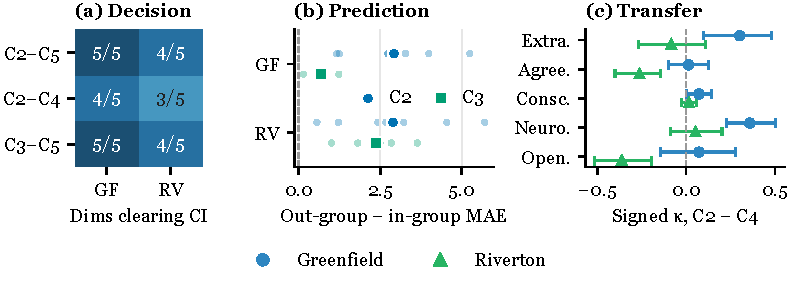
\includegraphics[width=\textwidth]{figures/fig6_route.pdf}
\caption{SCT route: clones diverge (a), predict exposed peers better (b), and transfer coherently (c).}\label{fig:route}
\end{figure}

\textbf{Finding 6 (RQ3): clones separate on the discussed task.} As Figure~\ref{fig:route}a shows, the $(C_2){-}(C_5)$ allocation contrast clears all five dimensions on Greenfield ($\bar g{=}{+}1.61$) and four of five on Riverton ($\bar g{=}{+}1.19$). The pure-interaction $(C_2){-}(C_4)$ row clears 4 of 5 dimensions on Greenfield and 3 of 5 on Riverton. This supports the SCT-Decision step. The agents first separate on the allocation problem, and the later off-topic probe is not an isolated psychometric blip.

\textbf{Finding 7 (RQ4): agents show an exposed-peer predictive advantage.} Each $C_2$ agent contributes one in-group MAE and one out-group MAE post-interaction. A one-sided paired Wilcoxon rejects the null in both scenarios. Greenfield has in-group MAE $4.18$ vs.\ out-group $7.10$ ($\Delta{=}{+}2.92$, $p{=}1.8{\times}10^{-8}$, $n{=}64$), and Riverton has $3.25$ vs.\ $6.15$ ($\Delta{=}{+}2.89$, $p{=}6.3{\times}10^{-10}$). The same contrast on $C_3$ is positive but smaller, with $\Delta{=}{+}0.69$ ($p{=}0.049$) and $\Delta{=}{+}2.36$ ($p{=}4.6{\times}10^{-5}$), as Figure~\ref{fig:route}b shows. The in-group target is an exposed peer, while the out-group target is absent from the predictor's conversation context. We therefore read this as an exposed-peer predictive advantage, with matched information access as the next control. Prediction is supporting evidence, and the primary BFI result stands on its own interaction control.

\textbf{Finding 8 (RQ5): the profile moves in coherent directions.} For each factor, $\kappa_f$ (Eq.~\ref{eq:drift}) compares post-minus-pre movement in $C_2$ and $C_4$ after reverse coding. Greenfield has $\kappa{=}{+}0.302$ for extraversion and ${+}0.358$ for neuroticism, both with 8/8 directional agreement across replicas, and ${+}0.072$ for conscientiousness with 7/8. Riverton has ${-}0.263$ for agreeableness (8/8) and ${-}0.362$ for openness (7/8), as Figure~\ref{fig:route}c shows. Greenfield's aggregate L1 variance ratio $C_2/C_4$ is 0.47, so its clearest factors move consistently while dispersion falls. Riverton's ratio is 4.11, a larger contribution from dispersion alongside consistent agreeableness and openness movement. The profile directions are therefore coherent and scenario-specific.

\subsection{RQ6: Does the Direction Hold Across Models, and What Does It Imply?}\label{sec:exp-cross}

\begin{figure}[t]
\centering
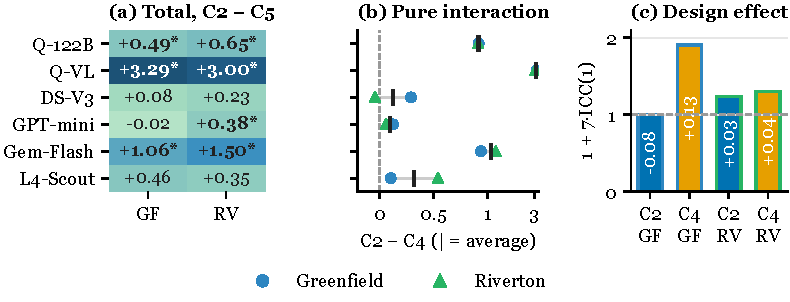
\includegraphics[width=\textwidth]{figures/fig7_breadth.pdf}
\caption{Cross-model breadth (a, b) and replicate dependence (c). All five $(C_2){-}(C_4)$ averages are positive.}\label{fig:breadth}
\end{figure}

\textbf{Finding 9: directional breadth is positive but uneven.} As Figure~\ref{fig:breadth}a shows, three of the five non-primary variants reach significance on $(C_2){-}(C_5)$ in at least one scenario. Qwen3-VL-32B and Gemini-2.5-Flash reach significance in both scenarios, and GPT-4.1-mini reaches significance on Riverton. DeepSeek-V3 and Llama-4-Scout do not reach significance. Under a no-effect null, ten scenario-by-variant cells tested at $\alpha{=}0.05$ would yield 0.5 positive cells in expectation. We observe five positive cells and no significant reversal. The smaller within-family Qwen3-VL-32B variant produces the largest raw drift ($\bar{\Delta}{\approx}3.0{-}3.3$), but its standardized $g$ is inflated by an unstable pooled SD on its own $C_5$ (Appendix~\ref{app:cross}).

\textbf{Finding 10: the pure-interaction contrast is positive for every variant on average.} We completed matched $(C_2){-}(C_4)$ runs for all five variants, three runs per condition and scenario (Figure~\ref{fig:breadth}b). All 5/5 model-level scenario averages are positive (one-sided exact sign test $p{=}0.031$). The panel includes DeepSeek-V3's near-zero, slightly reversed Riverton cell. A 3 vs.\ 3 two-sided exact permutation test has 20 possible allocations, so its minimum attainable $p$ is 0.10. The panel therefore provides directional breadth across the five tested controlled-clone configurations.

\textbf{Finding 11: uncertainty belongs at the simulation level.} OASIS-style populations are used to estimate group polarization and herd-effect trajectories, including normal-theory intervals over posts and comments within one simulated interaction process~\citep{OASIS}. Agents and posts that share an evolving history also share dependence. In our data, estimated agent-level ICC(1) ranges from $-0.079$ to $0.129$ across the four primary cells, and treating 8 agents as independent would overstate effective sample size by design factors up to 1.91 (Figure~\ref{fig:breadth}c). The practical correction is to keep the point estimate, recompute uncertainty at the independent simulation level, and check it against a no-interaction condition.

\subsection{RQ7: Does Transfer Extend Beyond BFI-10 in Riverton?}\label{sec:exp-scenario}\label{sec:exp-case}

\begin{table}[t]
\centering\footnotesize
\setlength{\tabcolsep}{3pt}
\caption{Gate status (A) and the Riverton route (B). BFI-10 is SCT-positive in both scenarios.}\label{tab:gates}\label{tab:riverton-case}
\begin{tabular}{l cc cc}
\toprule
\multicolumn{5}{l}{\textbf{(A) Gate status}, $\bar\Delta$ ($g$) with 95\% CI or Welch $p$} \\
& \multicolumn{2}{c}{Greenfield} & \multicolumn{2}{c}{Riverton} \\
\cmidrule(lr){2-3}\cmidrule(lr){4-5}
\tableinput{tables/t3_gates.tex}
\bottomrule
\end{tabular}

\vspace{4pt}
\begin{tabular}{P{0.13\textwidth}P{0.44\textwidth}P{0.38\textwidth}}
\toprule
\multicolumn{3}{l}{\textbf{(B) Riverton case study along the SCT route}} \\
Route step & Observed pattern & Interpretation \\
\midrule
Decision & $(C_2){-}(C_5)$ clears 4 of 5 allocation dimensions, $\bar g{=}{+}1.19$ & Interacting clones separate on the discussed budget task \\
Prediction & in-group MAE $3.25$ vs.\ out-group $6.15$, $\Delta{=}{+}2.89$, $p{=}6.3{\times}10^{-10}$ & Exposed-peer predictive advantage \\
Primary transfer & BFI-10 $(C_2){-}(C_4)$ gives $\bar{\Delta}{=}{+}0.91$, $g{=}{+}0.96$ & Off-topic response-profile drift survives the matched-brief control \\
Secondary transfer & conformity $g{=}{-}0.62$, consistency $g{=}{+}1.74$ on $(C_2){-}(C_4)$ & The strongest scenario also changes social-pressure and consistency probes \\
\bottomrule
\end{tabular}
\end{table}

\textbf{Finding 12: in Riverton, transfer extends beyond BFI-10.} The scenario asks an AI Transition Committee to allocate a \$5M budget across Automation, Workforce Training, Employee Support, Innovation Lab, and Data Infrastructure. Brief A emphasizes efficiency and technology infrastructure. Brief B emphasizes workforce readiness and employee support. Table~\ref{tab:gates}B shows how the same run family moves from topic-level divergence to peer modeling and then to off-topic transfer. Riverton is a boundary case, not a claim about all domains. Conformity is SCT-positive on Riverton but null on Greenfield ($g{=}{-}0.05$, $p{=}0.81$). Consistency on the same contrast is significantly positive on Riverton but null on Greenfield ($g{=}{+}0.01$). On Greenfield, the consistency lift on $(C_2){-}(C_5)$ is driven by the brief component $(C_4){-}(C_5)$ rather than by interaction. A reasonable account is that Riverton's workplace transition framing creates stronger group identification than Greenfield's community-grant framing, so effects that depend on in-group identification emerge more clearly. Wording consistency also concerns the allocation topic itself, so it cannot by itself establish off-topic transfer. We report the asymmetry rather than averaging it away.

\section{Limitations}\label{sec:exp-limits}

\textbf{Model and replica scope.} The within-Qwen3-122B-FP8 factorial uses one primary model. The five variants add $(C_2){-}(C_4)$ with three runs per condition, which gives directional breadth but no individually significant replication. Replica counts follow $\{C_1{=}7, C_2{=}8, C_3{=}5, C_4{=}5, C_5{=}3, C_6{=}5\}$. The $C_5{=}3$ floor limits every baseline-subtracted contrast, including $(C_4){-}(C_5)$, $(C_3){-}(C_5)$, the $(C_2){-}(C_5)$ gates, and the no-SRM check, and its allocation outputs repeat exactly across its three runs (Appendix~\ref{app:stats}). The headline $(C_2){-}(C_4)$ effect holds the brief fixed and does not depend on $C_5$. The $(C_2){-}(C_1)$ contrast varies brief-symmetry and topology jointly, so no topology claim follows. Agent count, horizon, and topology are fixed in the tested scope.

\textbf{Construct and time.} BFI-10 is validated on humans, not LLMs, so absolute drift lacks a calibrated psychological interpretation. Self-report inventories can be unreliable for LLMs and need not track behavior~\citep{Shu2024_PsychReliability,Gupta2024_SelfAssessment,Han2025_PersonalityIllusion}, and familiar inventories may appear in training data~\citep{Han2026_Contamination}. We therefore report response-profile drift rather than ``personality change'', keep the probe wording fixed because format alone changes outputs~\citep{Sclar2024_PromptFormat}, and read the profiles as role-conditioned behavior of the model~\citep{Shanahan2023}, not as the dispositions of people~\citep{Dillion2023}. Mathematical and logical accuracy are distinct capability endpoints that we do not measure. BFI-10 is measured immediately before and after interaction, so the evidence supports post-interaction transfer, and delayed retention needs a branch from a clean post-interaction checkpoint. Asch-style conformity items may not generalize to subtler social pressure. BFI-10 is manuscript-designated primary without external preregistration.

\textbf{Matching and mechanism.} Matching holds at the protocol level: scenario, clone identities, briefs, probe constructors, model identifier, and decoding configuration. Tokenizer revision, assembled token IDs, endpoint precision, and batch placement fall outside the historical record (Appendix~\ref{app:audit}). Prediction compares an exposed in-group peer with an absent out-group target, so information access differs across targets. The clone-agent setup does not cover settings where agents diverge during pretraining or fine-tuning.

\section{Conclusion}\label{sec:conclusion}
Controlled-clone agents are not independent replicates after 30 rounds of social interaction. They drift on probes unrelated to the topic of conversation, and the drift is about 0.92 BFI-10 L1 units at the run level ($g{\approx}1.0$), cross-scenario stable, and directionally broad across architecture variants. The five-condition factorial rules out brief-alone explanations for the headline contrast. The no-SRM ablation weakens the memory-extractor explanation and suggests that typed memory may partly stabilize agent state. The solo-generation control shows that extended generation and history contribute, with the social-interaction condition highest in both scenarios. The Decision, Prediction, and Transfer route gives the phenomenon a testable structure rather than treating it as an isolated psychometric change. Multi-agent evaluations should treat each interacting simulation as one replicate and compare it with paired no-interaction controls.

\label{main-text-end}
\clearpage
\begin{ack}
% Complete both declarations for all authors; the relevant window is the
% 36 months before submission. Do not infer that no support/conflicts exist.
\textbf{Funding.} Author-supplied funding and support statement pending.

\textbf{Competing interests.} Author-supplied competing-interest disclosure pending.
\end{ack}

\bibliographystyle{unsrtnat}
\bibliography{custom}
\clearpage
\appendix
\section{Scenarios, Briefs, Probes}\label{app:scenarios}\label{app:materials}
The supplementary package includes the exact source files for the two scenario stems, the A and B briefs, the condition configs, and the runtime probe constructors. Table~\ref{tab:scenario-materials} summarizes the materials so the allocation and prediction tasks are visible in the PDF.

\begin{table}[h]
\centering\footnotesize
\caption{Synthetic decision materials used in Greenfield and Riverton.}\label{tab:scenario-materials}
\setlength{\tabcolsep}{3pt}\renewcommand{\arraystretch}{1.15}
\begin{tabular}{P{0.10\textwidth}P{0.19\textwidth}P{0.09\textwidth}P{0.27\textwidth}P{0.22\textwidth}}
\toprule
Scenario & Decision setting & Budget & Allocation dimensions & Brief contrast \\
\midrule
Greenfield & Community Investment Committee & \$10M grant & Education, Healthcare, Green Spaces, Infrastructure, Economic Development & Education-oriented community data versus wellbeing, green-space, and mental-health data \\
Riverton & AI Transition Committee at a manufacturing and technology firm & \$5M transition budget & Automation, Workforce Training, Employee Support, Innovation Lab, Data Infrastructure & Efficiency and technology-infrastructure data versus workforce readiness and employee-support data \\
\bottomrule
\end{tabular}
\end{table}

\paragraph{Runtime allocation probe.} The runtime probe asks each agent to distribute 100 percentage points across the five scenario-specific areas. It requires one area per line in the form \texttt{Area: [number]\%} and asks for no commentary. This stricter probe is the one used for all allocation-vector scoring.

\paragraph{Runtime prediction probe.} The post-discussion prediction probe asks each agent to predict how a named target agent would distribute 100 percentage points across the same five areas. It uses the same one-line-per-area format and asks for no commentary. Prediction MAE is computed from these predicted vectors against the target agent's realized post-discussion allocation.

\paragraph{Off-topic transfer probes.} The BFI-10 probe follows the original short inventory and the PsychoBench LLM adaptation~\citep{Rammstedt2007_BFI10,PsychoBench}. The prompt asks for ten integer Likert ratings from 1 to 5 only, with no explanation. The conformity probe uses paired natural and majority-pressure responses over 15 items inspired by classic Asch-style conformity framing~\citep{Asch1956_Conformity}, with randomized order between phases. The consistency probe asks the same final-position question in three phrasings and scores average pairwise word overlap, following a lightweight CogMir-inspired probe design~\citep{CogMir}. These operational definitions take precedence over informal ``personality'' or ``agreement'' labels.

\section{Statistics, Calibration, and Provenance}\label{app:stats}\label{app:audit}

\begin{table}[h]
\centering\footnotesize
\caption{Scoring formulas for the five SocCogEval instruments.}\label{tab:metrics}
\setlength{\tabcolsep}{4pt}\renewcommand{\arraystretch}{1.15}
\resizebox{\textwidth}{!}{%
\begin{tabular}{llll}
\toprule
Instrument & Per-agent score $y_i$ & Range and direction & Test against contrast \\
\midrule
Allocation divergence & $|x_{i,j}^{A}-x_{i,j}^{B}|$ per dim $j$ & higher \(=\) more divergent & per-dim CI excludes 0, majority rule \\
Prediction MAE & $\mathrm{MAE}(\hat{x}_{i\to j}, x_j)$ & lower \(=\) better at modeling $j$ & Wilcoxon paired (in $<$ out) \\
BFI-10 L1 drift & $\sum_{f}|s_{i,f}^{\text{post}}-s_{i,f}^{\text{pre}}|$ & higher \(=\) more drift, 0 to 20 & run-level exact permutation \\
Conformity rate & $\#\{\text{switched to majority}\}/\#\text{eligible}$ & 0 to 1 & two-sample on per-agent $y_i$ \\
Consistency score & agreement across 3 phrasings & 0 to 1, higher \(=\) more consistent & two-sample on per-agent $y_i$ \\
\bottomrule
\end{tabular}}
\end{table}

\textbf{Original agent-level estimator.} The submitted analysis computed allocation divergence, BFI L1 drift, conformity rate, and consistency score per agent ($n{=}\text{reps}\times 8$ agent-observations per condition), and prediction MAE per (predictor, target) pair aggregated per predictor. CIs came from a two-level cluster bootstrap that resamples replicas with replacement and then agents within each sampled replica (10{,}000 resamples), with Welch's $t$ as the parametric reference. Table~\ref{tab:decomp-agent} keeps those values. The main text leads with the run-level exact tests in Table~\ref{tab:decomp}, whose point estimates are identical because every run has eight agents.

\begin{table}[h]
\centering\footnotesize
\setlength{\tabcolsep}{3.5pt}
\caption{BFI-10 decomposition with the original agent-stratified bootstrap and Welch $p$.}\label{tab:decomp-agent}
\resizebox{\textwidth}{!}{%
\begin{tabular}{ll ccc ccc}
\toprule
& & \multicolumn{3}{c}{Greenfield} & \multicolumn{3}{c}{Riverton} \\
\cmidrule(lr){3-5}\cmidrule(lr){6-8}
Contrast & Isolates & $\bar\Delta$ ($g$) & 95\% CI & $p$ & $\bar\Delta$ ($g$) & 95\% CI & $p$ \\
\midrule
\tableinput{tables/app_decomp_agent.tex}
\bottomrule
\end{tabular}}
\end{table}

\begin{table}[h]
\centering\footnotesize
\caption{Primary and solo-control BFI-10 run means, ordered by replica index.}\label{tab:runvalues}
\begin{tabular}{llP{0.64\linewidth}}
\toprule
Scenario & Condition & Run means \\
\midrule
\tableinput{tables/run_rows.tex}
\bottomrule
\end{tabular}
\end{table}

\begin{table}[h]
\centering\footnotesize
\caption{Dependence diagnostics on agent BFI L1 scores, with $\mathrm{DE}=1+7\max(0,\widehat{\mathrm{ICC}})$.}\label{tab:icc}
\begin{tabular}{llrrrr}
\toprule
Scenario & Condition & ICC(1) & DE & Nominal $n$ & Effective $n$ \\
\midrule
\tableinput{tables/icc_rows.tex}
\bottomrule
\end{tabular}
\end{table}

\textbf{Calibration.} Repeated SRM extractions on two pilot dialogues recover the same fields in all repeated runs, with 5 extractions per dialogue and a target of at least 90\%. Condition $C_4$ produces detectable allocation shifts on 2 of 5 dimensions in Greenfield and 4 of 5 dimensions in Riverton, leaving room for interaction effects to appear on top. Under $T{=}0.0$, $C_5$ produces zero allocation divergence on at least 3 of 5 dimensions in both scenarios. A temperature sweep confirms that increasing $T$ inflates the $C_5$ floor monotonically, supporting $T{=}0.0$ for deterministic instruments (Figure~\ref{F5}).

\begin{figure}[h]
\centering
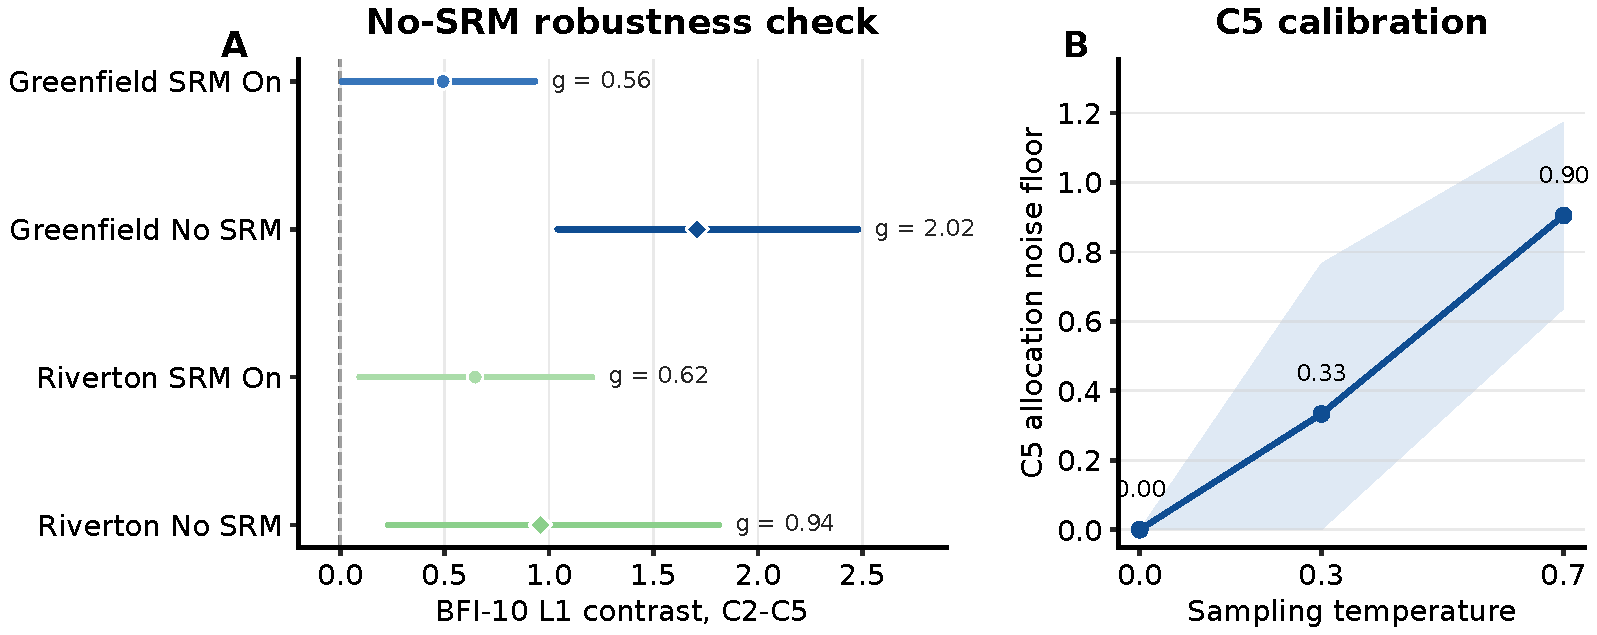
\includegraphics[width=0.92\textwidth]{figures/A2.pdf}
\caption{No-SRM robustness (left) and the $C_5$ calibration floor across temperature (right).}\label{F5}
\end{figure}

\textbf{Instrument-specific floor.} At BFI temperature 0.7, all three $C_5$ raw-response payloads and score payloads differ in each scenario. Agent pre/post score equality is 0.042 in Greenfield and 0.208 in Riverton. At allocation temperature zero, all three nominal $C_5$ runs have identical raw responses and allocation arrays, and every agent's allocation is unchanged pre/post. Repeating this deterministic payload contributes no new floor variation, which is why the $C_5$-dependent contrasts are qualified in Section~\ref{sec:exp-limits}.

\textbf{Provenance.} The release identifies every selected run and retains its configuration, pre/post measurements, and summary. The original 128-run ledger comprises 56 primary runs, 60 historical cross-variant $C_2/C_5$ runs, and 12 no-SRM runs. Thirty added cross-variant $C_4$ runs and ten formal $C_6$ runs bring the total to 168. Frozen-state temperature-zero probes reuse existing trajectories and do not increase the independent run count. The primary and $C_6$ intervals use 50,000 bootstrap draws with fixed seeds, and the other run-level intervals use the same estimator. For historical runs, exact request tokens, immutable provider revisions, tokenizer revisions, precision, batch placement, and run-time source commits are incompletely recorded. Source reconstruction establishes matching initial prompt construction for a corresponding named agent in $C_2$ and $C_4$. The post-treatment requests intentionally differ through stored interaction memory, and probes leave agent state unchanged in the current implementation.

\subsection{Compute and Reproduction}\label{app:cost}
Total wall-clock time on primary Qwen3-122B-FP8 (TP=2, both scenarios, 56 production runs, excluding the no-SRM robustness check) is approximately 90 GPU-hours on H200. The completed no-SRM check adds approximately 38 wall-clock hours on the same TP=2 server (about 76 additional H200 GPU-hours). Cross-architecture API runs incur single-digit dollar API fees. The local visual variant on Qwen3-VL-32B takes approximately 5 GPU-hours per scenario. These historical estimates do not cover the added $C_4$ runs, temperature re-probing, or $C_6$, whose audited call and token totals are in the artifact tables. The compact measurement package supports offline numerical verification without an LLM service. It includes selected run configurations, raw pre/post responses, derived scores, summaries, selection manifests, and hashes. Live regeneration additionally requires model weights or provider access and a recorded serving configuration.

\section{Matched Non-Social Control}\label{app:c6}
The $C_6$ design was frozen on 25 July 2026. Operational clarifications and a throughput amendment were recorded before formal outcomes were inspected. Each round has three generation stages and one extraction stage, with a barrier between stages. Each generation stage submits one independent call for every agent. Each agent sees its own current-round outputs, and previous rounds are accessed through the same memory interface as the interaction protocol. The first prompt asks for private reasoning about the allocation problem, values, evidence, and tradeoffs. The second asks the agent to reconsider that reasoning from another angle and resolve a tension or uncertainty. The third asks for its current best allocation reasoning and any change in its own view. All three prohibit addressing, quoting, predicting, or simulating another person.

Formal $C_6$ runs used tensor parallelism 1, maximum context length 8,192, FP8, eager execution, GPU memory utilization 0.92, and at most eight concurrent sequences. Two incomplete serial Greenfield attempts were operationally aborted and excluded, and all ten formal runs restarted under the amended serving schedule. Every audited formal run has 720 content calls and 240 extraction calls. $C_6$ records request and output hashes, serving metadata, and token counts. Historical $C_2$ did not save equivalent token usage, so we claim neither realized token equality nor a token-normalized social effect.

\subsection{Belief-Probe Time Course}\label{app:timecourse}
Belief probes run every five rounds and leave conversation history and memory unchanged. Their free text rarely states all five allocation shares (14\% of probes), so we track wording instead. For each run and probe round, \emph{wording separation} is the mean Jaccard word overlap between agents in the same group minus the mean overlap between agents in different groups, after removing stop words. Groups are agents 0--3 and 4--7, as in every other group-level analysis. Figure~\ref{fig:timecourse} uses the ledger-selected primary $C_1$, $C_2$, and $C_3$ runs and the ten $C_6$ runs, with run-bootstrap bands.

\begin{figure}[h]
\centering
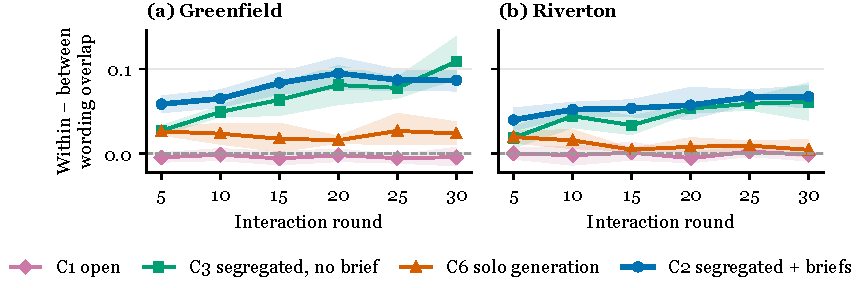
\includegraphics[width=\textwidth]{figures/time_course.pdf}
\caption{Within-group minus between-group wording overlap of belief probes over rounds.}\label{fig:timecourse}
\end{figure}

Within-group convergence grows over the episode in the two segregated interaction conditions. On Greenfield, separation moves from $+0.059$ to $+0.087$ in $C_2$ and from $+0.027$ to $+0.109$ in $C_3$ between rounds 5 and 30, and on Riverton from $+0.040$ to $+0.067$ and from $+0.019$ to $+0.061$. The solo-generation condition starts near the $C_3$ level because of its asymmetric briefs and then stays flat or declines ($+0.026$ to $+0.024$, and $+0.020$ to $+0.004$). The open-network $C_1$ stays at zero. Agents in segregated conditions talk only within their group, so part of this convergence is shared vocabulary from the conversations themselves. The measure is descriptive and is computed from stored probe text after the experiments.

\section{Cross-Variant Tables and Routing}\label{app:cross}\label{app:routing}

\begin{table}[h]
\centering\footnotesize
\setlength{\tabcolsep}{3.5pt}
\caption{BFI-10 L1 drift, $(C_2){-}(C_5)$, across model variants (original agent-level estimator).}\label{tab:cross}
\begin{tabular}{l ccc ccc c}
\toprule
& \multicolumn{3}{c}{Greenfield} & \multicolumn{3}{c}{Riverton} & Same dir \\
\cmidrule(lr){2-4}\cmidrule(lr){5-7}
Variant & $\bar{\Delta}$ & $g$ & $p$ & $\bar{\Delta}$ & $g$ & $p$ & GF, RV \\
\midrule
\tableinput{tables/app_cross_c2c5.tex}
\bottomrule
\multicolumn{8}{l}{\footnotesize $^{\dagger}$Raw $\bar{\Delta}$ is load-bearing. $g$ is inflated because the small-$n$ pooled SD on its $C_5$ approaches the floor.} \\
\end{tabular}
\end{table}

\begin{table}[h]
\centering\footnotesize
\caption{Additional variants, run-level $(C_2){-}(C_4)$, three runs per condition and scenario.}\label{tab:cross-c4}
\begin{tabular}{lrrr}
\toprule
Variant & Greenfield & Riverton & Scenario average \\
\midrule
\tableinput{tables/cross_rows.tex}
\bottomrule
\end{tabular}
\end{table}

The cross-variant analogue of Table~\ref{tab:cross} is provided for conformity and consistency per scenario per variant in the released analysis files. Conformity replication is mixed, with Gemini-2.5-Flash significant on Greenfield, GPT-4.1-mini significant on Riverton, and others mostly null. Consistency replication is broad, with 5 of 6 variants positive on Riverton and 3 of 6 on Greenfield, with no significant decrease anywhere. These $(C_2){-}(C_5)$ estimands are not pooled with the $(C_2){-}(C_4)$ panel.

Each additional-variant $C_2/C_4$ scenario cell contains three completed runs. Selection uses the last complete timestamped retry for each prescribed cell, as specified by the original cross-variant analysis, and all complete candidates remain listed. A completed cell with a reversed effect remains included. For DeepSeek-V3, historical $C_2$ configurations record \texttt{deepseek-chat}, while the selected $C_4$ runs record \texttt{deepseek-v4-flash}. Historical immutable revisions are not available, so we report the identifier difference without treating it as a verified same-revision experiment. Endpoint configuration used DeepSeek-V3, GPT-4.1-mini, Gemini-2.5-Flash, and Llama-4-Scout via provider APIs, with Llama-4-Scout routed through OpenRouter. The primary analysis filters cross-variant replicas out of the within-Qwen3-122B-FP8 factorial via run-id pattern. The sign summary averages the two scenario differences within each variant before counting directions, so ten scenario cells are not treated as ten independent models.

\section{Signed and Temperature Robustness}\label{app:signed}

\begin{table}[h]
\centering\footnotesize
\caption{Signed factor diagnostics $\kappa_f$, $C_2-C_4$, with run-bootstrap intervals (10,000 draws).}\label{tab:signed}
\begin{tabular}{llrrc}
\toprule
Scenario & Factor & $\kappa_f$ & 95\% interval & Agreement \\
\midrule
\tableinput{tables/signed_rows.tex}
\bottomrule
\end{tabular}
\end{table}

The deterministic re-probe uses the same ten BFI items and reverse-coding rules, replacing only probe temperature. Saved post-treatment states retain their history, so it is a sensitivity analysis over the same experimental trajectories rather than an independently generated replication. Factor analyses are descriptive and are not corrected for multiple comparisons, for example by false-discovery-rate control~\citep{Benjamini1995}. Figure~\ref{fig:app-part2-breakdown} gives the factor-level drift and the secondary Part 2 metrics from the original analysis.

\begin{figure}[h]
\centering
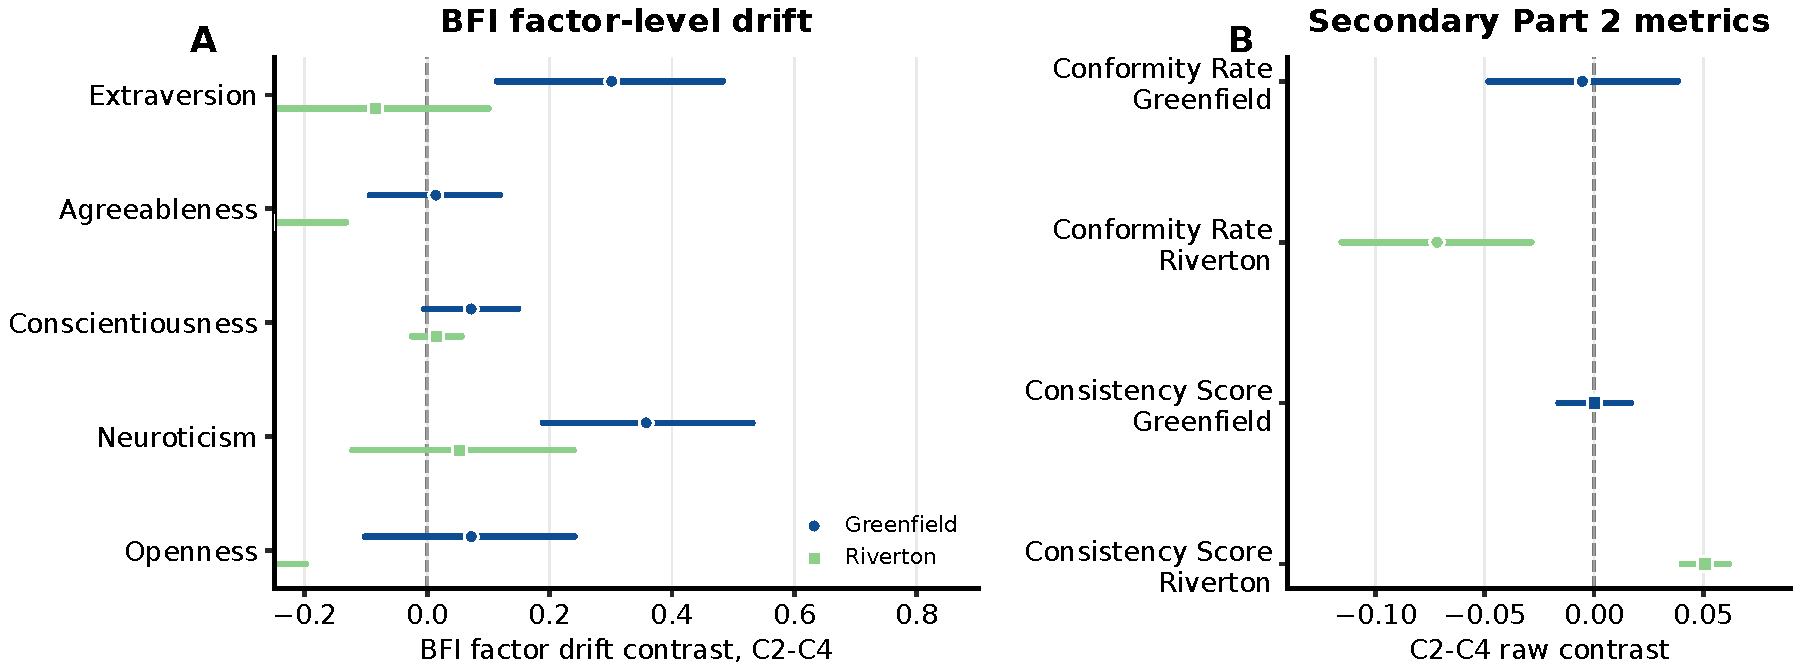
\includegraphics[width=0.92\textwidth]{figures/A3.pdf}
\caption{Part 2 breakdown: BFI-10 factor-level drift (left) and secondary metrics (right).}\label{fig:app-part2-breakdown}
\end{figure}

\section{Supporting Analyses}\label{app:secondary}

\begin{table}[h]
\centering\footnotesize
\caption{Verbatim-history no-SRM check, original agent-level estimator (3 vs.\ 3 replicas).}\label{tab:nosrm}
\resizebox{\textwidth}{!}{%
\begin{tabular}{lcccc}
\toprule
Scenario & $C_2$ mean & $C_5$ mean & $\bar{\Delta}$ ($g$) & 95\% CI, $p$ \\
\midrule
\tableinput{tables/app_nosrm_agent.tex}
\bottomrule
\end{tabular}}
\end{table}

No-SRM $C_2$ run means are $[2.000,2.250,3.188]$ in Greenfield and $[1.500,2.500,1.563]$ in Riverton, against $C_5$ means $[0.938,0.688,0.688]$ and $[1.125,1.063,0.500]$. Exact two-sided tests enumerate $\binom{6}{3}=20$ allocations and give $p=0.10$ in both cases, so the agent-level Welch values in Table~\ref{tab:nosrm} are not used as confirmatory evidence.

\begin{table}[h]
\centering\footnotesize
\begin{minipage}[t]{0.47\textwidth}\centering
\caption{Secondary $C_2-C_4$ summaries.}\label{tab:secondary}
\resizebox{\linewidth}{!}{%
\begin{tabular}{llrr}
\toprule
Scen. & Instrument & Diff. & 95\% CI \\
\midrule
\tableinput{tables/secondary_rows.tex}
\bottomrule
\end{tabular}}
\end{minipage}\hfill
\begin{minipage}[t]{0.5\textwidth}\centering
\caption{Per-dimension $C_2-C_4$ allocation (pp).}\label{tab:allocation}
\resizebox{\linewidth}{!}{%
\begin{tabular}{llrr}
\toprule
Scen. & Dimension & Diff. & 95\% CI \\
\midrule
\tableinput{tables/allocation_rows.tex}
\bottomrule
\end{tabular}}
\end{minipage}
\end{table}

\section{Extended Related Work}\label{app:related}
\textbf{Social influence before LLMs.} Repeated averaging of neighbors' opinions leads groups to consensus~\citep{DeGroot1974}, and later models keep a weight on each person's initial position while peers pull opinions together~\citep{Friedkin1990}. Experiments separate informational influence, where others count as evidence, from normative pressure to agree~\citep{Deutsch1955,Asch1956_Conformity}. Communication can also remove the diversity that makes independent judgments useful in aggregate~\citep{Lorenz2011}, and small committed minorities can tip a population's convention~\citep{Centola2018}. Similar convention dynamics appear in LLM populations~\citep{FlintAshery2025_Conventions}. Our segregated $C_2$ groups are a controlled version of this setting, with the off-topic BFI-10 probe asking whether influence extends past the discussed question.

\textbf{LLM agents as a study population.} Machine behavior has been proposed as an empirical science of individual and collective agent behavior~\citep{Rahwan2019}. Language models are used to simulate survey respondents and human-subject studies~\citep{Argyle2023,Aher2023_SimulateHumans}, generative agent-based models couple agent decisions with later interactions~\citep{Ghaffarzadegan2024}, and LLM simulations are argued to be a promising research method~\citep{Anthis2025_SocialSim}. Other work cautions that synthetic responses can misrepresent variation and mislead inference~\citep{Bisbee2024}, raises validity and reproducibility questions for generative social science~\citep{Bail2024}, and separates model responses from human participants~\citep{Dillion2023}. Treating each agent as one role a model plays~\citep{Shanahan2023} fits our reading of BFI-10 scores as response profiles. Close to our question, initially undifferentiated LLM agents develop distinct personalities through communication~\citep{Takata2024}. Our design adds a brief held fixed, matched no-interaction and solo-generation controls, and a transfer endpoint unrelated to the conversation.

\textbf{Measuring LLM personality.} Cognitive-psychology batteries characterize model behavior~\citep{Binz2023,CogBench}. Prompted personas can express target traits~\citep{Jiang2024_PersonaLLM}, and LLM-specific test sets aim at reliable and valid trait measurement~\citep{Lee2025_TRAIT}. Evidence on reliability is mixed. Some scales are consistent under tested conditions~\citep{Huang2024_ScaleReliability}, while other studies find unreliable answers, sensitivity to option order and prompt wording, and self-reports that do not predict behavior~\citep{Shu2024_PsychReliability,Gupta2024_SelfAssessment,Han2025_PersonalityIllusion,Sclar2024_PromptFormat}. Familiar inventories may also be contaminated~\citep{Han2026_Contamination}. We use BFI-10 as a fixed probe and compare its change across matched conditions, so a constant bias in the instrument cancels in the contrast. We do not claim that the inventory measures an LLM's personality.

\textbf{Influence and agreement in multi-agent LLM systems.} Debate can improve factuality and reasoning~\citep{Du2024_MultiagentDebate} and encourage divergent thinking~\citep{Liang2024_DivergentDebate}, and debating evaluators change each other's judgments~\citep{Chan2024_ChatEval}. Models agree with users and peers~\citep{Sharma2024_Sycophancy,Cheng2025_ELEPHANT}, defer to agents presented as authorities~\citep{Choi2026_Authority}, and conform to a majority~\citep{Weng2025_Conformity}. Interacting LLMs revise funding allocations in ways shaped by past opinions~\citep{CisnerosVelarde2025_Funding}. Multi-agent failures are often coordination and verification errors~\citep{Cemri2025_MASFailures}, and reliability drops over long conversations~\citep{Laban2025_LostMultiTurn}. These studies measure behavior inside the interaction. SocCogEval measures what the interaction leaves behind on an unrelated probe, and the solo-generation control separates partner effects from extended generation.

\textbf{Inference with dependent units.} When one unit's treatment affects another's outcome, causal estimands must be defined over exposure structures~\citep{Hudgens2008,Aronow2017}. Our estimand is defined at the run level, where the whole group receives the interaction treatment. Treating observations within one unit as replicates is pseudoreplication~\citep{Hurlbert1984}, cluster-robust inference is fragile with few clusters~\citep{Cameron2015}, and evaluation items that share a source need clustered errors~\citep{Miller2024_ErrorBars}. With 3 to 8 runs per cell, we use exact permutation over all allocations~\citep{Phipson2010}, run-bootstrap intervals~\citep{Efron1979}, and Hedges' bias-corrected $g$~\citep{Hedges1981} as a secondary scale.

\clearpage
\section*{NeurIPS Paper Checklist}




\begin{enumerate}

\item {\bf Claims}
    \item[] Question: Do the main claims made in the abstract and introduction accurately reflect the paper's contributions and scope?
    \item[] Answer: \answerYes{}
    \item[] Justification: Sections~\ref{sec:intro}--\ref{sec:exp-limits} state the tested scope, raw effects, run-level inference, and the unresolved social-versus-solo difference.
    \item[] Guidelines:
    \begin{itemize}
        \item The answer \answerNA{} means that the abstract and introduction do not include the claims made in the paper.
        \item The abstract and/or introduction should clearly state the claims made, including the contributions made in the paper and important assumptions and limitations. A \answerNo{} or \answerNA{} answer to this question will not be perceived well by the reviewers. 
        \item The claims made should match theoretical and experimental results, and reflect how much the results can be expected to generalize to other settings. 
        \item It is fine to include aspirational goals as motivation as long as it is clear that these goals are not attained by the paper. 
    \end{itemize}

\item {\bf Limitations}
    \item[] Question: Does the paper discuss the limitations of the work performed by the authors?
    \item[] Answer: \answerYes{}
    \item[] Justification: Section~\ref{sec:exp-limits} discusses construct, temporal, matching, sample-size, model-revision, and generalization limits.
    \item[] Guidelines:
    \begin{itemize}
        \item The answer \answerNA{} means that the paper has no limitation while the answer \answerNo{} means that the paper has limitations, but those are not discussed in the paper. 
        \item The authors are encouraged to create a separate ``Limitations'' section in their paper.
        \item The paper should point out any strong assumptions and how robust the results are to violations of these assumptions (e.g., independence assumptions, noiseless settings, model well-specification, asymptotic approximations only holding locally). The authors should reflect on how these assumptions might be violated in practice and what the implications would be.
        \item The authors should reflect on the scope of the claims made, e.g., if the approach was only tested on a few datasets or with a few runs. In general, empirical results often depend on implicit assumptions, which should be articulated.
        \item The authors should reflect on the factors that influence the performance of the approach. For example, a facial recognition algorithm may perform poorly when image resolution is low or images are taken in low lighting. Or a speech-to-text system might not be used reliably to provide closed captions for online lectures because it fails to handle technical jargon.
        \item The authors should discuss the computational efficiency of the proposed algorithms and how they scale with dataset size.
        \item If applicable, the authors should discuss possible limitations of their approach to address problems of privacy and fairness.
        \item While the authors might fear that complete honesty about limitations might be used by reviewers as grounds for rejection, a worse outcome might be that reviewers discover limitations that aren't acknowledged in the paper. The authors should use their best judgment and recognize that individual actions in favor of transparency play an important role in developing norms that preserve the integrity of the community. Reviewers will be specifically instructed to not penalize honesty concerning limitations.
    \end{itemize}

\item {\bf Theory assumptions and proofs}
    \item[] Question: For each theoretical result, does the paper provide the full set of assumptions and a complete (and correct) proof?
    \item[] Answer: \answerNA{}
    \item[] Justification: The work reports empirical experiments and descriptive statistical estimands, not theoretical results.
    \item[] Guidelines:
    \begin{itemize}
        \item The answer \answerNA{} means that the paper does not include theoretical results. 
        \item All the theorems, formulas, and proofs in the paper should be numbered and cross-referenced.
        \item All assumptions should be clearly stated or referenced in the statement of any theorems.
        \item The proofs can either appear in the main paper or the supplemental material, but if they appear in the supplemental material, the authors are encouraged to provide a short proof sketch to provide intuition. 
        \item Inversely, any informal proof provided in the core of the paper should be complemented by formal proofs provided in appendix or supplemental material.
        \item Theorems and Lemmas that the proof relies upon should be properly referenced. 
    \end{itemize}

    \item {\bf Experimental result reproducibility}
    \item[] Question: Does the paper fully disclose all the information needed to reproduce the main experimental results of the paper to the extent that it affects the main claims and/or conclusions of the paper (regardless of whether the code and data are provided or not)?
    \item[] Answer: \answerNo{}
    \item[] Justification: The accompanying measurements and scripts reproduce the reported outcome analysis. Exact regeneration is limited by missing historical serving revisions and token traces, as disclosed in Appendix~\ref{app:audit}.
    \item[] Guidelines:
    \begin{itemize}
        \item The answer \answerNA{} means that the paper does not include experiments.
        \item If the paper includes experiments, a \answerNo{} answer to this question will not be perceived well by the reviewers: Making the paper reproducible is important, regardless of whether the code and data are provided or not.
        \item If the contribution is a dataset and\slash or model, the authors should describe the steps taken to make their results reproducible or verifiable. 
        \item Depending on the contribution, reproducibility can be accomplished in various ways. For example, if the contribution is a novel architecture, describing the architecture fully might suffice, or if the contribution is a specific model and empirical evaluation, it may be necessary to either make it possible for others to replicate the model with the same dataset, or provide access to the model. In general. releasing code and data is often one good way to accomplish this, but reproducibility can also be provided via detailed instructions for how to replicate the results, access to a hosted model (e.g., in the case of a large language model), releasing of a model checkpoint, or other means that are appropriate to the research performed.
        \item While NeurIPS does not require releasing code, the conference does require all submissions to provide some reasonable avenue for reproducibility, which may depend on the nature of the contribution. For example
        \begin{enumerate}
            \item If the contribution is primarily a new algorithm, the paper should make it clear how to reproduce that algorithm.
            \item If the contribution is primarily a new model architecture, the paper should describe the architecture clearly and fully.
            \item If the contribution is a new model (e.g., a large language model), then there should either be a way to access this model for reproducing the results or a way to reproduce the model (e.g., with an open-source dataset or instructions for how to construct the dataset).
            \item We recognize that reproducibility may be tricky in some cases, in which case authors are welcome to describe the particular way they provide for reproducibility. In the case of closed-source models, it may be that access to the model is limited in some way (e.g., to registered users), but it should be possible for other researchers to have some path to reproducing or verifying the results.
        \end{enumerate}
    \end{itemize}


\item {\bf Open access to data and code}
    \item[] Question: Does the paper provide open access to the data and code, with sufficient instructions to faithfully reproduce the main experimental results, as described in supplemental material?
    \item[] Answer: \answerNo{}
    \item[] Justification: A publication package containing code, selected measurements, hashes, and offline reproduction instructions has been prepared. A permanent public repository URL and license have not yet been finalized.
    \item[] Guidelines:
    \begin{itemize}
        \item The answer \answerNA{} means that paper does not include experiments requiring code.
        \item Please see the NeurIPS code and data submission guidelines (\url{https://neurips.cc/public/guides/CodeSubmissionPolicy}) for more details.
        \item While we encourage the release of code and data, we understand that this might not be possible, so \answerNo{} is an acceptable answer. Papers cannot be rejected simply for not including code, unless this is central to the contribution (e.g., for a new open-source benchmark).
        \item The instructions should contain the exact command and environment needed to run to reproduce the results. See the NeurIPS code and data submission guidelines (\url{https://neurips.cc/public/guides/CodeSubmissionPolicy}) for more details.
        \item The authors should provide instructions on data access and preparation, including how to access the raw data, preprocessed data, intermediate data, and generated data, etc.
        \item The authors should provide scripts to reproduce all experimental results for the new proposed method and baselines. If only a subset of experiments are reproducible, they should state which ones are omitted from the script and why.
        \item At submission time, to preserve anonymity, the authors should release anonymized versions (if applicable).
        \item Providing as much information as possible in supplemental material (appended to the paper) is recommended, but including URLs to data and code is permitted.
    \end{itemize}


\item {\bf Experimental setting/details}
    \item[] Question: Does the paper specify all the training and test details (e.g., data splits, hyperparameters, how they were chosen, type of optimizer) necessary to understand the results?
    \item[] Answer: \answerYes{}
    \item[] Justification: Sections~\ref{sec:method} and~\ref{sec:fsip-cycle} specify conditions, agent counts, rounds, probes, temperatures, and contrasts. The frozen C6 protocol and serving amendment are included.
    \item[] Guidelines:
    \begin{itemize}
        \item The answer \answerNA{} means that the paper does not include experiments.
        \item The experimental setting should be presented in the core of the paper to a level of detail that is necessary to appreciate the results and make sense of them.
        \item The full details can be provided either with the code, in appendix, or as supplemental material.
    \end{itemize}

\item {\bf Experiment statistical significance}
    \item[] Question: Does the paper report error bars suitably and correctly defined or other appropriate information about the statistical significance of the experiments?
    \item[] Answer: \answerYes{}
    \item[] Justification: Section~\ref{sec:metrics} defines run-level exact tests and descriptive bootstrap intervals. Secondary estimates and small-cell limitations are labeled separately.
    \item[] Guidelines:
    \begin{itemize}
        \item The answer \answerNA{} means that the paper does not include experiments.
        \item The authors should answer \answerYes{} if the results are accompanied by error bars, confidence intervals, or statistical significance tests, at least for the experiments that support the main claims of the paper.
        \item The factors of variability that the error bars are capturing should be clearly stated (for example, train/test split, initialization, random drawing of some parameter, or overall run with given experimental conditions).
        \item The method for calculating the error bars should be explained (closed form formula, call to a library function, bootstrap, etc.)
        \item The assumptions made should be given (e.g., Normally distributed errors).
        \item It should be clear whether the error bar is the standard deviation or the standard error of the mean.
        \item It is OK to report 1-sigma error bars, but one should state it. The authors should preferably report a 2-sigma error bar than state that they have a 96\% CI, if the hypothesis of Normality of errors is not verified.
        \item For asymmetric distributions, the authors should be careful not to show in tables or figures symmetric error bars that would yield results that are out of range (e.g., negative error rates).
        \item If error bars are reported in tables or plots, the authors should explain in the text how they were calculated and reference the corresponding figures or tables in the text.
    \end{itemize}

\item {\bf Experiments compute resources}
    \item[] Question: For each experiment, does the paper provide sufficient information on the computer resources (type of compute workers, memory, time of execution) needed to reproduce the experiments?
    \item[] Answer: \answerNo{}
    \item[] Justification: Appendix~\ref{app:materials} reports available historical compute estimates and the C6 exposure accounting. A reconciled project-wide total including all added, failed, and pilot runs is unavailable.
    \item[] Guidelines:
    \begin{itemize}
        \item The answer \answerNA{} means that the paper does not include experiments.
        \item The paper should indicate the type of compute workers CPU or GPU, internal cluster, or cloud provider, including relevant memory and storage.
        \item The paper should provide the amount of compute required for each of the individual experimental runs as well as estimate the total compute. 
        \item The paper should disclose whether the full research project required more compute than the experiments reported in the paper (e.g., preliminary or failed experiments that didn't make it into the paper). 
    \end{itemize}
    
\item {\bf Code of ethics}
    \item[] Question: Does the research conducted in the paper conform, in every respect, with the NeurIPS Code of Ethics \url{https://neurips.cc/public/EthicsGuidelines}?
    \item[] Answer: \answerYes{}
    \item[] Justification: The study uses synthetic scenarios and LLM agents, without human participants or personal participant data. Construct limits and intended use are discussed in the paper.
    \item[] Guidelines:
    \begin{itemize}
        \item The answer \answerNA{} means that the authors have not reviewed the NeurIPS Code of Ethics.
        \item If the authors answer \answerNo, they should explain the special circumstances that require a deviation from the Code of Ethics.
        \item The authors should make sure to preserve anonymity (e.g., if there is a special consideration due to laws or regulations in their jurisdiction).
    \end{itemize}


\item {\bf Broader impacts}
    \item[] Question: Does the paper discuss both potential positive societal impacts and negative societal impacts of the work performed?
    \item[] Answer: \answerYes{}
    \item[] Justification: Section~\ref{sec:exp-limits} describes the uncertainty-estimation benefit and cautions against treating simulated profiles as measurements of real people.
    \item[] Guidelines:
    \begin{itemize}
        \item The answer \answerNA{} means that there is no societal impact of the work performed.
        \item If the authors answer \answerNA{} or \answerNo, they should explain why their work has no societal impact or why the paper does not address societal impact.
        \item Examples of negative societal impacts include potential malicious or unintended uses (e.g., disinformation, generating fake profiles, surveillance), fairness considerations (e.g., deployment of technologies that could make decisions that unfairly impact specific groups), privacy considerations, and security considerations.
        \item The conference expects that many papers will be foundational research and not tied to particular applications, let alone deployments. However, if there is a direct path to any negative applications, the authors should point it out. For example, it is legitimate to point out that an improvement in the quality of generative models could be used to generate Deepfakes for disinformation. On the other hand, it is not needed to point out that a generic algorithm for optimizing neural networks could enable people to train models that generate Deepfakes faster.
        \item The authors should consider possible harms that could arise when the technology is being used as intended and functioning correctly, harms that could arise when the technology is being used as intended but gives incorrect results, and harms following from (intentional or unintentional) misuse of the technology.
        \item If there are negative societal impacts, the authors could also discuss possible mitigation strategies (e.g., gated release of models, providing defenses in addition to attacks, mechanisms for monitoring misuse, mechanisms to monitor how a system learns from feedback over time, improving the efficiency and accessibility of ML).
    \end{itemize}
    
\item {\bf Safeguards}
    \item[] Question: Does the paper describe safeguards that have been put in place for responsible release of data or models that have a high risk for misuse (e.g., pre-trained language models, image generators, or scraped datasets)?
    \item[] Answer: \answerNA{}
    \item[] Justification: The release consists of experiment code and synthetic-agent measurements, not pretrained weights, scraped personal data, or a high-risk generative model.
    \item[] Guidelines:
    \begin{itemize}
        \item The answer \answerNA{} means that the paper poses no such risks.
        \item Released models that have a high risk for misuse or dual-use should be released with necessary safeguards to allow for controlled use of the model, for example by requiring that users adhere to usage guidelines or restrictions to access the model or implementing safety filters. 
        \item Datasets that have been scraped from the Internet could pose safety risks. The authors should describe how they avoided releasing unsafe images.
        \item We recognize that providing effective safeguards is challenging, and many papers do not require this, but we encourage authors to take this into account and make a best faith effort.
    \end{itemize}

\item {\bf Licenses for existing assets}
    \item[] Question: Are the creators or original owners of assets (e.g., code, data, models), used in the paper, properly credited and are the license and terms of use explicitly mentioned and properly respected?
    \item[] Answer: \answerNo{}
    \item[] Justification: Instrument and model sources are cited. The release documents third-party dependencies and source attributions; a complete asset-license audit and project licensing declaration remain to be finalized by the authors.
    \item[] Guidelines:
    \begin{itemize}
        \item The answer \answerNA{} means that the paper does not use existing assets.
        \item The authors should cite the original paper that produced the code package or dataset.
        \item The authors should state which version of the asset is used and, if possible, include a URL.
        \item The name of the license (e.g., CC-BY 4.0) should be included for each asset.
        \item For scraped data from a particular source (e.g., website), the copyright and terms of service of that source should be provided.
        \item If assets are released, the license, copyright information, and terms of use in the package should be provided. For popular datasets, \url{paperswithcode.com/datasets} has curated licenses for some datasets. Their licensing guide can help determine the license of a dataset.
        \item For existing datasets that are re-packaged, both the original license and the license of the derived asset (if it has changed) should be provided.
        \item If this information is not available online, the authors are encouraged to reach out to the asset's creators.
    \end{itemize}

\item {\bf New assets}
    \item[] Question: Are new assets introduced in the paper well documented and is the documentation provided alongside the assets?
    \item[] Answer: \answerYes{}
    \item[] Justification: Appendix~\ref{app:materials} and the accompanying README and data documentation describe the code, measurements, manifests, analysis commands, and reproducibility boundaries.
    \item[] Guidelines:
    \begin{itemize}
        \item The answer \answerNA{} means that the paper does not release new assets.
        \item Researchers should communicate the details of the dataset\slash code\slash model as part of their submissions via structured templates. This includes details about training, license, limitations, etc. 
        \item The paper should discuss whether and how consent was obtained from people whose asset is used.
        \item At submission time, remember to anonymize your assets (if applicable). You can either create an anonymized URL or include an anonymized zip file.
    \end{itemize}

\item {\bf Crowdsourcing and research with human subjects}
    \item[] Question: For crowdsourcing experiments and research with human subjects, does the paper include the full text of instructions given to participants and screenshots, if applicable, as well as details about compensation (if any)? 
    \item[] Answer: \answerNA{}
    \item[] Justification: There were no human participants or crowdsourcing workers.
    \item[] Guidelines:
    \begin{itemize}
        \item The answer \answerNA{} means that the paper does not involve crowdsourcing nor research with human subjects.
        \item Including this information in the supplemental material is fine, but if the main contribution of the paper involves human subjects, then as much detail as possible should be included in the main paper. 
        \item According to the NeurIPS Code of Ethics, workers involved in data collection, curation, or other labor should be paid at least the minimum wage in the country of the data collector. 
    \end{itemize}

\item {\bf Institutional review board (IRB) approvals or equivalent for research with human subjects}
    \item[] Question: Does the paper describe potential risks incurred by study participants, whether such risks were disclosed to the subjects, and whether Institutional Review Board (IRB) approvals (or an equivalent approval/review based on the requirements of your country or institution) were obtained?
    \item[] Answer: \answerNA{}
    \item[] Justification: The experiments involve synthetic LLM agents and no human subjects.
    \item[] Guidelines:
    \begin{itemize}
        \item The answer \answerNA{} means that the paper does not involve crowdsourcing nor research with human subjects.
        \item Depending on the country in which research is conducted, IRB approval (or equivalent) may be required for any human subjects research. If you obtained IRB approval, you should clearly state this in the paper. 
        \item We recognize that the procedures for this may vary significantly between institutions and locations, and we expect authors to adhere to the NeurIPS Code of Ethics and the guidelines for their institution. 
        \item For initial submissions, do not include any information that would break anonymity (if applicable), such as the institution conducting the review.
    \end{itemize}

\item {\bf Declaration of LLM usage}
    \item[] Question: Does the paper describe the usage of LLMs if it is an important, original, or non-standard component of the core methods in this research? Note that if the LLM is used only for writing, editing, or formatting purposes and does \emph{not} impact the core methodology, scientific rigor, or originality of the research, declaration is not required.
    %this research? 
    \item[] Answer: \answerYes{}
    \item[] Justification: LLMs are the experimental agents. Their roles, recorded model identifiers, prompts, decoding settings, and routing limitations are described in Sections~\ref{sec:method} and~\ref{sec:fsip-cycle} and Appendix~\ref{app:routing}.
    \item[] Guidelines:
    \begin{itemize}
        \item The answer \answerNA{} means that the core method development in this research does not involve LLMs as any important, original, or non-standard components.
        \item Please refer to our LLM policy in the NeurIPS handbook for what should or should not be described.
    \end{itemize}

\end{enumerate}
\end{document}
